% Template for Elsevier CRC journal article
% version 1.2 dated 09 May 2011

% This file (c) 2009-2011 Elsevier Ltd.  Modifications may be freely made,
% provided the edited file is saved under a different name

% This file contains modifications for Transportation Research Procedia

% Changes since version 1.1
% - added "procedia" option compliant with ecrc.sty version 1.2a
%   (makes the layout approximately the same as the Word CRC template)
% - added example for generating copyright line in abstract

%-----------------------------------------------------------------------------------

%% This template uses the elsarticle.cls document class and the extension package ecrc.sty
%% For full documentation on usage of elsarticle.cls, consult the documentation "elsdoc.pdf"
%% Further resources available at http://www.elsevier.com/latex

%-----------------------------------------------------------------------------------

%%%%%%%%%%%%%%%%%%%%%%%%%%%%%%%%%%%%%%%%%%%%%%%%%%%%%%%%%%%%%%
%%%%%%%%%%%%%%%%%%%%%%%%%%%%%%%%%%%%%%%%%%%%%%%%%%%%%%%%%%%%%%
%%                                                          %%
%% Important note on usage                                  %%
%% -----------------------                                  %%
%% This file should normally be compiled with PDFLaTeX      %%
%% Using standard LaTeX should work but may produce clashes %%
%%   Please see      www.cirpe2026.com                      %%
%%%%%%%%%%%%%%%%%%%%%%%%%%%%%%%%%%%%%%%%%%%%%%%%%%%%%%%%%%%%%%
%%%%%%%%%%%%%%%%%%%%%%%%%%%%%%%%%%%%%%%%%%%%%%%%%%%%%%%%%%%%%%

%% The '3p' and 'times' class options of elsarticle are used for Elsevier CRC
%% The 'procedia' option causes ecrc to approximate to the Word template
\documentclass[5p,times,procedia]{elsarticle}
\flushbottom

%% The `ecrc' package must be called to make the CRC functionality available
\usepackage{ecrc}
%\usepackage{amsmath}


%% The ecrc package defines commands needed for running heads and logos.
%% For running heads, you can set the journal name, the volume, the starting page and the authors

%% set the volume if you know. Otherwise `00'
\volume{00}

%% set the starting page if not 1
\firstpage{1}

%% Give the name of the journal
\journalname{Procedia CIRP}

%% Give the author list to appear in the running head
%% Example \runauth{C.V. Radhakrishnan et al.}
\runauth{Mansfeldt et al.}

%% The choice of journal logo is determined by the \jid and \jnltitlelogo commands.
%% A user-supplied logo with the name <\jid>logo.pdf will be inserted if present.
%% e.g. if \jid{yspmi} the system will look for a file yspmilogo.pdf
%% Otherwise the content of \jnltitlelogo will be set between horizontal lines as a default logo

%% Give the abbreviation of the Journal.
\jid{trpro}

%% Give a short journal name for the dummy logo (if needed)
%\jnltitlelogo{Transportation Research}

%% Hereafter the template follows `elsarticle'.
%% For more details see the existing template files elsarticle-template-harv.tex and elsarticle-template-num.tex.

%% Elsevier CRC generally uses a numbered reference style
%% For this, the conventions of elsarticle-template-num.tex should be followed (included below)
%% If using BibTeX, use the style file elsarticle-num.bst

%% End of ecrc-specific commands
%%%%%%%%%%%%%%%%%%%%%%%%%%%%%%%%%%%%%%%%%%%%%%%%%%%%%%%%%%%%%%%%%%%%%%%%%%

%% The amssymb package provides various useful mathematical symbols

\usepackage{amssymb}
%% The amsthm package provides extended theorem environments
%% \usepackage{amsthm}

%% The lineno packages adds line numbers. Start line numbering with
%% \begin{linenumbers}, end it with \end{linenumbers}. Or switch it on
%% for the whole article with \linenumbers after \end{frontmatter}.
%% \usepackage{lineno}

%% natbib.sty is loaded by default. However, natbib options can be
%% provided with \biboptions{...} command. Following options are
%% valid:

%%   round  -  round parentheses are used (default)
%%   square -  square brackets are used   [option]
%%   curly  -  curly braces are used      {option}
%%   angle  -  angle brackets are used    <option>
%%   semicolon  -  multiple citations separated by semi-colon
%%   colon  - same as semicolon, an earlier confusion
%%   comma  -  separated by comma
%%   numbers-  selects numerical citations
%%   super  -  numerical citations as superscripts
%%   sort   -  sorts multiple citations according to order in ref. list
%%   sort&compress   -  like sort, but also compresses numerical citations
%%   compress - compresses without sorting
%%
\biboptions{sort&compress}

% \biboptions{}

% if you have landscape tables
\usepackage[figuresright]{rotating}
%\usepackage{harvard}
% put your own definitions here:x
%   \newcommand{\cZ}{\cal{Z}}
%   \newtheorem{def}{Definition}[section]
%   ...

% add words to TeX's hyphenation exception list
%\hyphenation{author another created financial paper re-commend-ed Post-Script}

% declarations for front matter

\usepackage[bookmarks=false]{hyperref}
    \hypersetup{colorlinks,
      linkcolor=blue,
      citecolor=blue,
      urlcolor=blue}

% additional packages
\usepackage{todonotes}
\newcommand{\iltodo}[2][]{\todo[inline, #1]{#2}}
\usepackage{cleveref}
\usepackage{booktabs}
\usepackage{multirow}

\begin{document}
\begin{frontmatter}

%% Title, authors and addresses

%% use the tnoteref command within \title for footnotes;
%% use the tnotetext command for the associated footnote;
%% use the fnref command within \author or \address for footnotes;
%% use the fntext command for the associated footnote;
%% use the corref command within \author for corresponding author footnotes;
%% use the cortext command for the associated footnote;
%% use the ead command for the email address,
%% and the form \ead[url] for the home page:
%%
%% \title{Title\tnoteref{label1}}
%% \tnotetext[label1]{}
%% \author{Name\corref{cor1}\fnref{label2}}
%% \ead{email address}
%% \ead[url]{home page}
%% \fntext[label2]{}
%% \cortext[cor1]{}
%% \address{Address\fnref{label3}}
%% \fntext[label3]{}

\dochead{14th CIRP Global Web Conference (CIRPe 2026)}%

\title{Comparison of CAD Model Representations for Machine Learning: Guidance for Representation Selection}

%% use optional labels to link authors explicitly to addresses:
%% \author[label1,label2]{<author name>}
%% \address[label1]{<address>}
%% \address[label2]{<address>}



\author[a,b]{Daniel Mansfeldt\corref{cor1}} 
\author[a,b]{Michel Kruse}
\author[a,b]{Lasse Päplow}
\author[a]{Max Brede}
\author[b]{Daniel Böhnke}
%\ead{author@institute.xxx}

\address[a]{F\&E GmbH, Schwentinestr. 24, 24149 Kiel, Germany}
\address[b]{Institut für Produktionstechnik und CIMTT der HAW Kiel, Schwentinestr. 13, 24149 Kiel, Germany}

\cortext[cor1]{* Corresponding author. {\it E-mail address:} daniel.mansfeldt@haw-kiel.de}

\begin{abstract}
%% Text of abstract
Selecting an appropriate representation for CAD data processing remains a fundamental challenge, as it requires balancing geometric accuracy with computational efficiency for downstream tasks.
While representations such as voxels, point clouds and meshes have been extensively studied in the context of 3D machine learning, representations such as dimensionless invariants, STEP file-based trees, and vector sets represent comparatively recent approaches.
Each of these new approaches is rooted in a distinct and widely adopted paradigm — descriptors, graphs, and neural fields, respectively.
This paper presents a structured comparison of these approaches, including voxel as a strong baseline, evaluating them on classification and regression tasks using the \textit{FabWave} dataset.
The authors aim to characterize the strengths and limitations of each approach, providing actionable guidance on selecting a representation suited to specific tasks.
\end{abstract}

\begin{keyword}
CAD; 3D Model Representation; Machine Learning; Classification; Regression; Comparison 

%% keywords here, in the form: keyword \sep keyword

%% PACS codes here, in the form: \PACS code \sep code

%% MSC codes here, in the form: \MSC code \sep code
%% or \MSC[2008] code \sep code (2000 is the default)

\end{keyword}
%\cortext[cor1]{Corresponding author. Tel.: +0-000-000-0000 ; fax: +0-000-000-0000.}

\end{frontmatter}

%%
%% Start line numbering here if you want
%%
% \linenumbers

%% main text

%\enlargethispage{-7mm}
\section{Introduction}\label{sec:Introduction}
A wide variety of machine learning (ML) architectures have been developed to handle the many possible representations of geometric data.
Each representation requires its custom ML architecture to be processible in the first place.
This means that a variety of representations and their corresponding model layouts must be compared when developing a new application to determine the most suitable one. 

Geometric data can be conveyed using a variety of representations.
These include multi-view images~\cite{kanezaki2018rotationnet}, voxels~\cite{liu2019point-voxel,wang2019normalnet}, point clouds~\cite{qi2016pointnet}, meshes~\cite{pernot2015thin} and graphs~\cite{miles2023recursive}, among others.
The different representations of essentially the same information require the use of a variety of ML-based approaches for CAD data analysis. 

Unfortunately, each representation has its own advantages and disadvantages.
Voxels, for instance, limit the maximum resolution of CAD models because the number of voxels grows cubically, while computing resources remain limited.
This makes it challenging to choose the best representation form and associated ML model for a given task.
To help guide the decision on which data representation form to use, we compare five promising machine learning approaches, each using a distinct 3D data representation.

By comparing these approaches using general CAD attributes—rather than attributes tailored to specific production use cases—we identify which machine learning models, together with their respective input data representations, are likely to perform well across a broad range of applications.
To ensure a fair comparison, all models are trained and tested on the same dataset.
Specifically, we use the \textit{FabWave} dataset~\cite{starly2019fabwave} and preprocess it to enable comparison across the different approaches.

Our contributions include: 
\begin{itemize}
    \item Comparison of five different CAD model representation forms, including dimensionless invariants, trees extracted from \mbox{B-Rep} models (here applied to STEP files), multi-view images and vector sets.
    \item Performance comparison of data representation and ML model combinations for the classification of real engineering parts.
    \item Performance comparison of data representation and ML model combinations for regression tasks aimed at predicting basic properties of real engineering parts.
\end{itemize}

Our work is subject to the following limitations:
\begin{itemize}
    \item The application of a certain representation requires a specific ML model architecture. Therefore, we cannot compare the representation forms independently of the ML models.
    \item Only a subset of the available CAD model representation forms and ML architectures is considered. 
\end{itemize}

The rest of this paper is structured as follows.
In \cref{sec:Related-Work}, we review related work. This includes the foundations of the ML models examined and the CAD model representation types used.
\Cref{sec:Methodology} presents our methodology for preparing the data set and comparing model performance.
\Cref{sec:results-and-discussion} presents our results and discusses their implications.
Finally, \cref{sec:conclusion-and-future-works} provides a conclusion and lists possible future works. 

The code and resources used in this study are publicly available at: \url{https://github.com/CIMTT-Kiel/cad-representation-selection}.

\section{Related Work}\label{sec:Related-Work}
As we aim to determine the best pair of CAD model representation and ML architecture, we lay out the different representation schemes and ML architectures considered.

Note that these do not encompass all available approaches, but rather a selection of promising methods.
Other approaches the reader may be interested in include \textit{\mbox{UV-Net}}~\cite{jayaraman2021uv}, \textit{\mbox{PointNet}}~\cite{qi2016pointnet} and \textit{\mbox{MeshCNN}}~\cite{hanocka2019meshcnn}, among others.

\subsection{Representation of 3D CAD Models for Processing via Machine Learning Models}\label{sec:CAD-Representations}
Research on 3D data representations for machine learning has explored a wide range of approaches, including point clouds, pure primitive instancing, cell decomposition, constructive solid geometry, sweep representations and boundary representations (B-Reps)~\cite{requicha1980representations}.
Although each representation scheme is suitable for certain use cases, not all of them can be processed directly by a given machine learning model.

To address this limitation, several techniques have been developed to derive machine-learning-compatible data structures from CAD models while preserving relevant topological and geometric information.
In this work, we utilize five such techniques, each of which is described in detail below.
To the best of our knowledge, these 3D data representation techniques have not previously been compared with respect to a geometry analysis use case.

\subsubsection{Voxels}\label{sec:CAD-Representations-Voxels}
Representing 3D data as voxels is the least complex form of cell decomposition.
Here, the 3D space is discretized into a regular grid of cubic cells, where each cell (voxel) is assigned a binary value indicating whether it is occupied by the object or not.
This representation can be directly processed by convolutional neural networks (CNNs).

One disadvantage of voxel representations is that they can require a large amount of memory, especially for high-resolution models, due to the cubic growth in the number of voxels with increasing resolution. This can lead to computational inefficiency and may limit the level of detail that can be captured in the model.~\cite{requicha1980representations}

\subsubsection{Images}\label{sec:CAD-Representations-Images}
CAD models can be transformed into sets of images suitable for processing by machine learning models.
Since convolutional neural networks are widely used for image analysis, this approach offers a straightforward and practical solution.

However, adequate representation of a CAD model requires images from a sufficiently large number of viewpoints.
If the number of views is too limited, relevant geometric features may not be captured.
This challenge is particularly pronounced for internal features, which cannot be observed from external viewpoints alone.
Although this limitation can be mitigated by incorporating cross-sectional images taken at multiple slice positions, doing so significantly increases the number of required images and, consequently, the computational cost.
Therefore, an appropriate balance must be found between representational fidelity and computational efficiency. 

Several prior studies have employed image-based approaches for CAD model analysis~\cite{kanezaki2018rotationnet,li2023multi}. 

\subsubsection{Tree Data Structure}\label{sec:CAD-Representations-Tree}
Miles et al.\ emphasize that \mbox{B-Rep} models possess an inherent hierarchical structure.
For instance, a line is defined by a point and a direction vector.
Based on this property, topological entities such as vertices, edges, and faces can be modeled as a graph, with geometric information incorporated through coordinate-based attributes.
Such a representation is well suited for the application of graph neural networks to CAD models.~\cite{miles2023recursive}

\subsubsection{Dimensionless Invariants}\label{sec:CAD-Representations-Dimensionless-Invariants}
Another approach to obtain an encoding vector was introduced by Kaiser et al.\ based on the Pi-Theorem~\cite{kaiser2018automated}.
They argue that any three-dimensional body can be described by a set of dimensionless invariants.
To derive them from a CAD model, the geometry is first discretized based on the \mbox{B-Rep} into a volume mesh.
Statistical moments $\mu_{pqr} = \int_V x^p y^q z^r \, \mathrm{d}V$ are then computed by
numerical integration over the elements, and the Buckingham Pi-theorem is applied leading to a compact vector of dimensionless and thus scale-invariant features.

To establish a meaningful connection between feature vectors across different geometries, it is necessary to ensure uniform location and orientation. With these regularized feature vectors, morphological similarity can be reduced to a distance metric. Topological information of the \mbox{B-Rep} such as connectivity between faces, edges or vertices is lost during discretization. Additionally, the automated meshing of datasets with variable geometric characteristics represents a notable limitation of this approach. The meshing process may fail for certain geometries or may require part-specific considerations.

Nevertheless, the compact vectors offer a key advantage, enabling highly efficient storage and retrieval at scale.

\subsubsection{Vecset}\label{sec:CAD-Representations-Vecset}
Recent advances in 3D representation learning have explored a range of approaches.
While classical methods rely on explicit representations such as meshes~\cite{bronstein2009discrete} or rasterized structures like voxel~\cite{wang2019normalnet} or octrees~\cite{tang1992octree}, the geometric neural field approach~\cite{chen2019learning,park2019deepsdf} encodes shapes as continuous functions represented by the network itself.
This leads to a high training effort for large amounts of data and to a lack of a regularized latent representation, due to the separately trained and thereby shape-specific networks.

To bridge this gap, 3DShape2VecSet~\cite{zhang20233dshape2vecset} introduces a hybrid approach that represents shapes as sets of latent vectors (VecSets), thereby decoupling shape-specific information into learnable vector sets while maintaining a single network across all shapes.
It employs cross-attention mechanisms to query spatial coordinates, achieving a compact yet expressive shape encoding.
This design enables efficient integration with generative models, particularly diffusion models~\cite{zhang20233dshape2vecset}, allowing for tasks such as unconditional generation, text-conditioned synthesis and shape completion.  

\subsection{Architecture of Machine Learning Models for CAD Model Processing}\label{sec:ML-Architectures}
Different CAD model representations require different machine learning architectures to process them.
This section introduces the architectures considered in this work. 

\subsubsection{Multilayer Perceptron}\label{sec:ML-Architectures-MLP}
Multilayer perceptrons (MLPs), also referred to as feedforward neural networks, are among the most fundamental architectures in deep learning.
For single-vector inputs, MLPs can be used for both classification and regression.
In this work, they are therefore employed to make predictions from invariant representations and vector sets. 

MLPs are also frequently integrated into more specialized machine learning architectures.
For example, they are commonly used as prediction heads, where they take the output vector of a preceding model component as input and produce the final prediction vector.
In this capacity, MLPs are also used as components of the other architectures evaluated in this paper. 

\subsubsection{Child-Sum Tree-LSTM}\label{sec:ML-Architectures-TreeLSTM}
Miles et al.\ used a Child-Sum Tree-LSTM~\cite{tai2015improved} to generate encoding vectors for CAD models~\cite{miles2023recursive}.
The model recursively traverses the tree structure of the CAD representation and computes, at each node, an encoding vector for the corresponding topological entity.
This computation combines the entity type represented by the node with the sum of its children's encoding vectors via LSTM gating.
Through this recursive aggregation, the Child-Sum Tree-LSTM produces a single encoding vector for the entire CAD model, which can subsequently be used as input to a range of downstream machine learning models.

\subsubsection{Convolutional Neural Network}\label{sec:ML-Architectures-CNN}
Convolutional neural networks (CNNs) are a class of machine learning architectures widely employed in image processing tasks.
They typically comprise convolutional and pooling layers that learn local image features.
These features are subsequently passed to a MLP, which generates the final prediction~\cite{james2013introduction}.

As voxel representations (see \cref{sec:CAD-Representations-Voxels}) are defined on regular grid structures, \mbox{3D-CNNs} can be applied to such representations directly.

Pretrained architectures such as YOLO are commonly used for object detection and image classification~\cite{redmon2016you}.
In contrast to YOLO, which operates on a single input image, multi-view architectures such as \textit{RotationNet}~\cite{kanezaki2018rotationnet} process multiple images to produce a single prediction.

\section{Methodology}\label{sec:Methodology}
\subsection{Data Set}\label{sec:Methodology-Data-Set}
We use the FabWave dataset~\cite{starly2019fabwave} to benchmark the proposed models.
The dataset contains a broad range of CAD models, predominantly representing mechanical components.
In its original form, it comprises more than 4,000 parts in STEP format assigned to 44 object categories.

Before the dataset could be used for model training and evaluation, extensive preprocessing was required.
The individual preprocessing steps are described below. 

First, the dataset was filtered.
Some CAD models contained overlapping or disjoint bodies, which could not be converted into all representations considered in this work.
These models were therefore either fused into a single closed shell or removed from the dataset.
In addition, object classes containing fewer than ten CAD models were excluded. 

Second, the different representations as described in the following \cref{sec:Methodology-Representations} were generated for each remaining CAD model.
If a representation could not be generated for a given CAD model, the model was excluded from the dataset entirely.
This ensured that all remaining CAD models could be processed by all evaluated approaches, enabling a fair comparison of their performance.

Third, the target values were derived for each CAD model.
These targets included the part class, the volume and the numbers of faces, edges and vertices. 
For scaling, the natural logarithm was applied to the numerical target values before training the machine learning models.

Fourth, the data splits were prepared. The dataset was divided into training, validation and test sets using stratified sampling to keep the class distribution consistent across all splits.

Finally, to reduce class imbalance, the training split was oversampled such that each class contained at least half of the median class size. Validation and test splits were left unchanged. \Cref{tab:data-splits} provides details for the absolute split sizes.

\begin{table}[h]
\caption{Data Splits: Metadata for the training, validation and test splits of the preprocessed dataset.}
\label{tab:data-splits}
\begin{tabular*}{\hsize}{@{\extracolsep{\fill}}lrr@{}}
\toprule
    Data Split & Target fraction & Total Number of Samples\\
    \hline
    Training & 0.6 & 1662\\
    Validation & 0.2 & 518\\
    Test & 0.2 & 520\\
\botrule
\end{tabular*}
\end{table}

\subsection{Generation of the Representations}\label{sec:Methodology-Representations}
All representations were derived from the same filtered set of STEP files as described in~\cref{sec:Methodology-Data-Set}.

For the voxel representation, each model was tessellated and voxelized into a binary grid of $128^3$~cells.
The voxel size was chosen such that the longest extent of the part spans the grid, and the occupied region was centred within it.

For the image representation, 20 orthographic views of $224\times224$ pixels were rendered per part, with the camera positions distributed evenly over a sphere, matching the viewpoint configuration of RotationNet~\cite{kanezaki2018rotationnet}.

For the tree representation, the STEP file was parsed directly into a graph of topological entities following Miles et\ al.~\cite{miles2023recursive}, with entity types encoded as one-hot node labels.

For the vecset representation, $8192$ points were sampled uniformly from the model surface, centred and scaled to the unit sphere, and encoded into a set of $1024$ latent vectors of dimension 32 using the pretrained encoder of Zhang et al.~\cite{zhang20233dshape2vecset}.

For the invariant representation, the \mbox{B-Rep} was discretized into a tetrahedral mesh, which was centred and rotated by a principal component analysis such that the direction of largest variance is aligned with the $x$-axis and the second-largest with the $y$-axis.
On this mesh, 19 moments were computed by numerical quadrature. The specific choice of exponent triples is documented in the accompanying repository. Applying the Pi-theorem, each moment was normalized by the second-order moments:

\begin{equation}
\pi_{pqr} = \frac{\mu_{pqr}}{\mu_{200}^{\frac{4p-q-r+2}{10}}\,\mu_{020}^{\frac{4q-p-r+2}{10}}\,\mu_{002}^{\frac{4r-q-p+2}{10}}}
\end{equation}

This leads to three trivial quantities $\pi_{200}=\pi_{020}=\pi_{002}=1$. These are discarded, leaving a feature vector of size $16$.

\subsection{Approach Comparison}\label{sec:Methodology-Model-Comparison}
We compare the evaluated representations in combination with the corresponding ML models separately for the classification and regression tasks.

In the classification task, the machine learning models distinguish between $25$ object classes.
Ideally, abstract model categories would be used to assess the generalization capabilities of the models more broadly.
However, defining complex abstract CAD models while assigning them to meaningful and consistent classes remains challenging.
We therefore use the object classes provided by the FabWave dataset.

Since the dataset primarily contains mechanical engineering components, the resulting assessment is most directly applicable to CAD model analysis in the mechanical engineering domain.
Nevertheless, the results also provide insights into the applicability of the models to other 3D CAD analysis tasks, albeit to a lesser extent. 

Classification performance is evaluated using accuracy, $F_1$ score, recall, and precision.
The latter three metrics are \mbox{macro-averaged} across all classes to account for class-level performance independently of class frequency.
In addition, confusion matrices are provided to enable a more detailed comparison of the model's performance on individual classes. 

The regression task aims to predict abstract and generally available properties of CAD models.
Accordingly, the target quantities include the volume and the numbers of vertices, edges, and faces.
These properties can be computed for \mbox{B-Rep} CAD models independently of their domain or specific use case, making them suitable for evaluating the broader applicability of the ML models.

These tasks should be understood as a measure of information preservation rather than of geometric reasoning in isolation. A target that is explicitly contained in a representation is therefore expected to be predicted well by design, so the comparison is most informative for those representations in which the target is not directly available. Table~\ref{tab:encoding} summarizes how each target is encoded in each representation. Note that the volume is discarded by all representations that normalize the model to a fixed extent during conversion. The predictions of this target therefore rely on size being inferable from shape within the dataset.

\begin{table}[h]
\caption{Encoding of the Regression Targets. The table indicates whether a target is explicitly contained in the input (E), implicitly derivable (I), or discarded during conversion (L).}
\label{tab:encoding}
\begin{tabular*}{\columnwidth}{@{\extracolsep{\fill}}lccccc@{}}
\hline
Target & Voxel & Images & Trees & Invariants & Vecsets \\
\hline
Volume & L & L & I & L & L \\
Faces & I & I & E & I & I \\
Edges & I & I & E & I & I \\
Vertices & I & I & E & I & I \\
\hline
\end{tabular*}
\end{table}

RotationNet is not considered for the regression task, as it was originally designed for classification.
Although adapting RotationNet for regression appears feasible, such a modification is outside the scope of this work. 

As voxel representations are the least complex representation form considered in this work, they are used as a baseline.

\section{Results and Discussion}\label{sec:results-and-discussion}
This section presents the results of the comparison between the different CAD analysis approaches.
Classification and regression results are reported and interpreted separately.

Note that the observed ranking reflects the performance of the combination of representation and ML model.
It cannot be attributed solely to either the representation or the model.

Please refer to \labelcref{sec:appendix} for all diagrams referenced in this section.

\subsection{Classification}\label{sec:results-classification}

\Cref{fig:classification-metrics} and \cref{tab:classification-metrics} summarize the overall classification performance of the different approaches.

The \mbox{tree-based} approach achieves the best performance for all evaluated metrics and therefore can be regarded as the dominant approach for the classification task. 

Nevertheless, the other approaches may still achieve sufficiently high performance for practical application, depending on the specific requirements of a given use case.
In particular, they may be preferable if other factors, such as computational efficiency, implementation complexity, or data availability, outweigh the observed loss in prediction quality.

\begin{table}[h]
\caption{Classification Metrics: Listing of \mbox{macro-averaged} classification metric values as visualised in \cref{fig:classification-metrics}. The highest value per metric is highlighted in bold font.}
\label{tab:classification-metrics}
\begin{tabular*}{\hsize}{@{\extracolsep{\fill}}lcccc@{}}
\toprule
    Model & Accuracy & $F_1$ Score & Recall & Precision \\
    \midrule
    Vecsets     & 0.9519            & 0.9364            & 0.9509            & 0.9315 \\
    Trees       & \textbf{0.9750}   & \textbf{0.9565}   & \textbf{0.9583}   & \textbf{0.9549} \\
    Images      & 0.9462            & 0.9361            & 0.9447            & 0.9361 \\
    Invariants  & 0.7519            & 0.7857            & 0.7968            & 0.8174 \\
    Voxel       & 0.8865            & 0.8430            & 0.8555            & 0.8600 \\
\bottomrule
\end{tabular*}
\end{table}

To set the classification results into context, we also evaluated a dummy classifier that randomly predicts classes based on their frequency in the corresponding data split, see \cref{fig:dummy-classifier}.

\Cref{fig:confusion-matrix-trees,fig:confusion-matrix-images,fig:confusion-matrix-invariants,fig:confusion-matrix-vecset,fig:confusion-matrix-voxels} show the confusion matrices for all approaches.
Each one manages to recognize most classes with accuracies close to one.
Considering the overall classification metrics, this was to be expected.
Concurrently the image and tree approaches each fail to recognize one class entirely, the invariant-based approach two: it assigns all rollers and all bearings to washers. Together with the confusion between o-rings and washers, this indicates that the classes it confuses are all flat rotationally symmetric parts differing mainly in absolute size.

The tree-based approach misclassifies all bearings as washers.
We hypothesize that the encoding vector generated by the Child-Sum Tree-LSTM focuses primarily on macroscopic geometric features while potentially overlooking scale-dependent characteristics.
This may explain the confusion between bearings and washers: both are predominantly circular components with a central hole, but they differ in scale.

\subsection{Regression}\label{sec:results-regression}
\Cref{tab:regression} summarizes the regression results with reference baselines. As the targets are strongly right-skewed, the metrics need not agree on a ranking. The global baselines are constant predictors fitted on the global target distribution. The class-conditional predicts the median of the true class indicating what is attainable from class membership. Absolute scores are therefore of limited value on their own. Only the margin over the baselines can be attributed to the geometric information in the representation.

\Cref{fig:error-distributions} shows the distributions of the relative errors for the regression target quantities.
It should be noted that the displayed violin areas are affected by the logarithmic scale and are therefore not directly comparable in terms of absolute area.
As in the classification task, the \mbox{tree-based} approach achieves the best overall performance compared with the other approaches.

This conclusion is also supported by MAE, MSE and $R^2$ in \cref{tab:regression}, with the exception of the volume target, where the tree-based approach ranks second behind the invariant-based one. Its advantage on the three topological targets is expected by design, as predicting them reduces to counting the nodes of the input graph (see \cref{tab:encoding}).

For the volume target, the invariant representation is strictly scale-invariant and carries no absolute size information, so the high $R^2$ cannot be attributed to the input encoding. The oracle baseline already reaches $R^2 = 0.739$, so part size is largely inferable from part class within FabWave. This also shows that $R^2$ discriminates poorly for this target, as it is dominated by a few large parts. In terms of relative error, which is not affected by this imbalance, the tree-based approach leads on the volume target as well, with a median of $0.23$ against $0.66$ for the invariant-based approach and $0.82$ for the oracle baseline.

On the topological targets, the oracle already predicts $68\%$ of the test parts exactly, as many FabWave classes are topologically homogeneous and vary only in dimension. Differences between the approaches on these targets therefore reflect class recognition to a large extent, and only the margin over the oracle indicates what is inferred from the geometry itself.

The \mbox{invariant-based} approach attains slightly lower medians, but with substantially heavier tails. Its mean relative errors exceed those of the \mbox{tree-based} approach by roughly a factor of six. The \mbox{tree-based} approach therefore remains the most reliable across all regression targets.


\section{Conclusion and Future Works}\label{sec:conclusion-and-future-works}
We compared five machine learning approaches for CAD model analysis.
Each approach was evaluated on the FabWave dataset~\cite{starly2019fabwave} using a classification task with high class diversity, as well as several abstract regression tasks.

The results show that the combination of tree-structured graph representations and a Child-Sum Tree-LSTM model, as proposed by Miles et\ al.~\cite{miles2023recursive}, achieves the best performance across all evaluated tasks.
We therefore conclude that this method provides a promising starting point for more specialized CAD model analysis applications.
Nevertheless, the other approaches produced comparable results in some cases and may also be suitable, particularly when considerations other than predictive performance favor them over the \mbox{tree-based} approach.

Future work should investigate the performance of the \mbox{tree-based} method on additional datasets.
In particular, constructing datasets with more abstract learning tasks could help further demonstrate the model's general applicability. 

The generalization capabilities of the evaluated methods could also be explored by incorporating additional features into the comparison, such as bounding box dimensions, \mbox{surface-to-volume} ratio or shape complexity.

%\iltodo{decide on what to write here}
%Acknowledgements and Reference heading should be left justified, bold, with the first letter capitalized but have no numbers. Text below continues as normal.

%% The Appendices part is started with the command \appendix;
%% appendix sections are then done as normal sections
%% \appendix

%% \section{}
%% \label{}

\appendix
\section{Results Diagrams}
\label{sec:appendix}
The appendix contains all diagrams referenced in \cref{sec:results-and-discussion}.

% Classification metrics plot
\begin{figure*}[h] 
\centerline{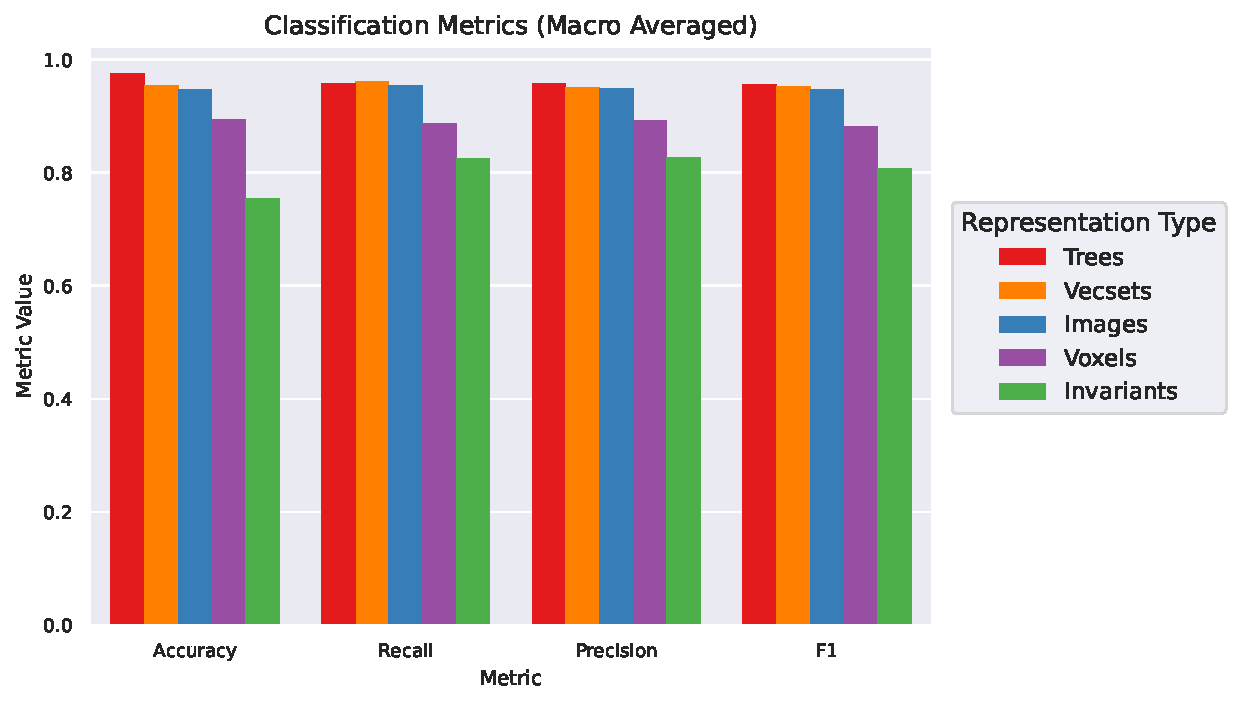
\includegraphics[width=0.9\textwidth]{classification_metrics_plot.pdf}}
\caption{\textbf{Classification Metrics}\\Comparison of the different approaches in terms of overall accuracy and macro-averaged $F_1$ score, recall and precision. The tree representation and associated Child-Sum Tree-LSTM model is dominating the others across all metrics.}
\label{fig:classification-metrics}
\end{figure*}

\begin{figure*}[h]
\centerline{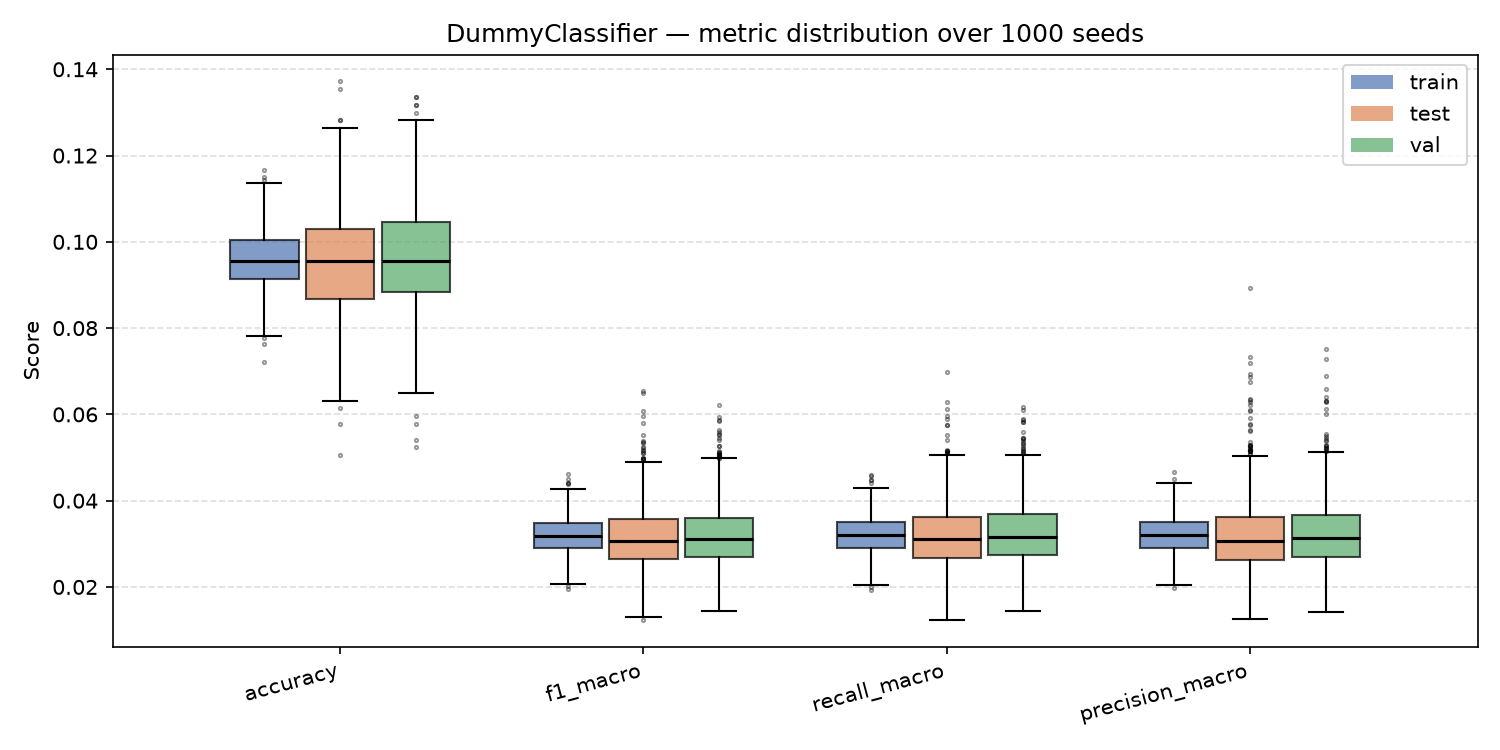
\includegraphics[width=0.9\textwidth]{clf_stability.png}}
\caption{\textbf{Dummy Classifier}\\The plot shows the performance of a dummy classifier that randomly predicts classes based on their frequency in the corresponding data split. The distributions of the results are shown for 1000 different random seeds. For each metric, similar results are obtained for the training, validation and test splits.}
\label{fig:dummy-classifier}
\end{figure*}

% Confusion matrices
\begin{figure*}[h]\vspace*{4pt}
\centerline{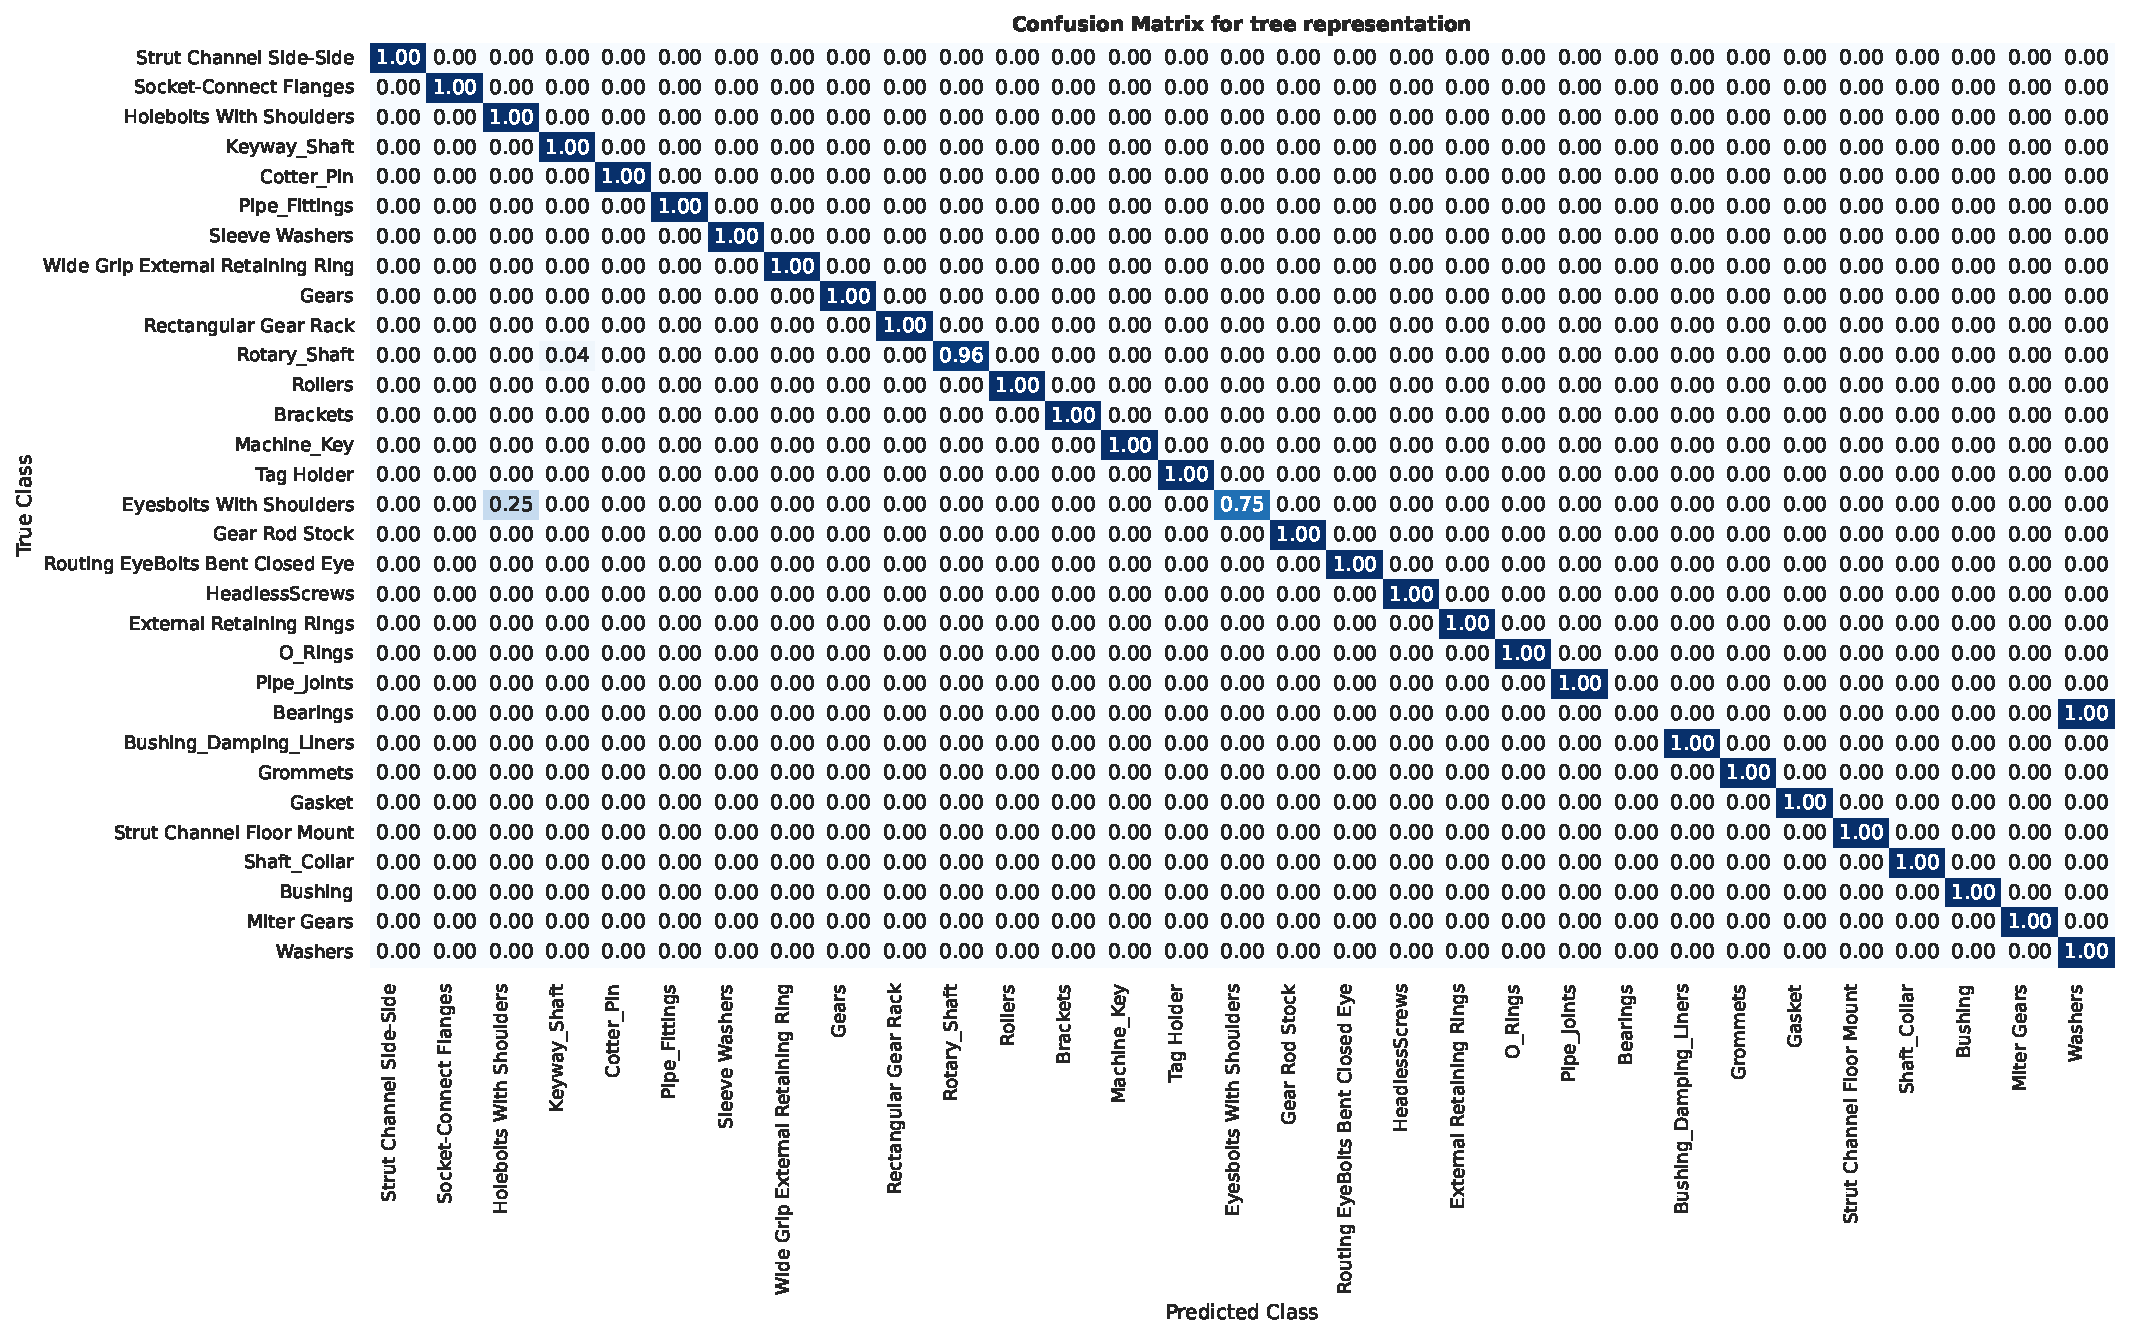
\includegraphics[width=0.9\textwidth]{confusion_matrix_trees.pdf}}
\caption{\textbf{Confusion Matrix for the tree-based Approach}\\For each part class, the confusion matrix shows the distribution of predicted classes. The tree-based approach predicts most classes with high accuracy, but it confuses all bearings with washers.}
\label{fig:confusion-matrix-trees}
\end{figure*}

\begin{figure*}[h]
\centerline{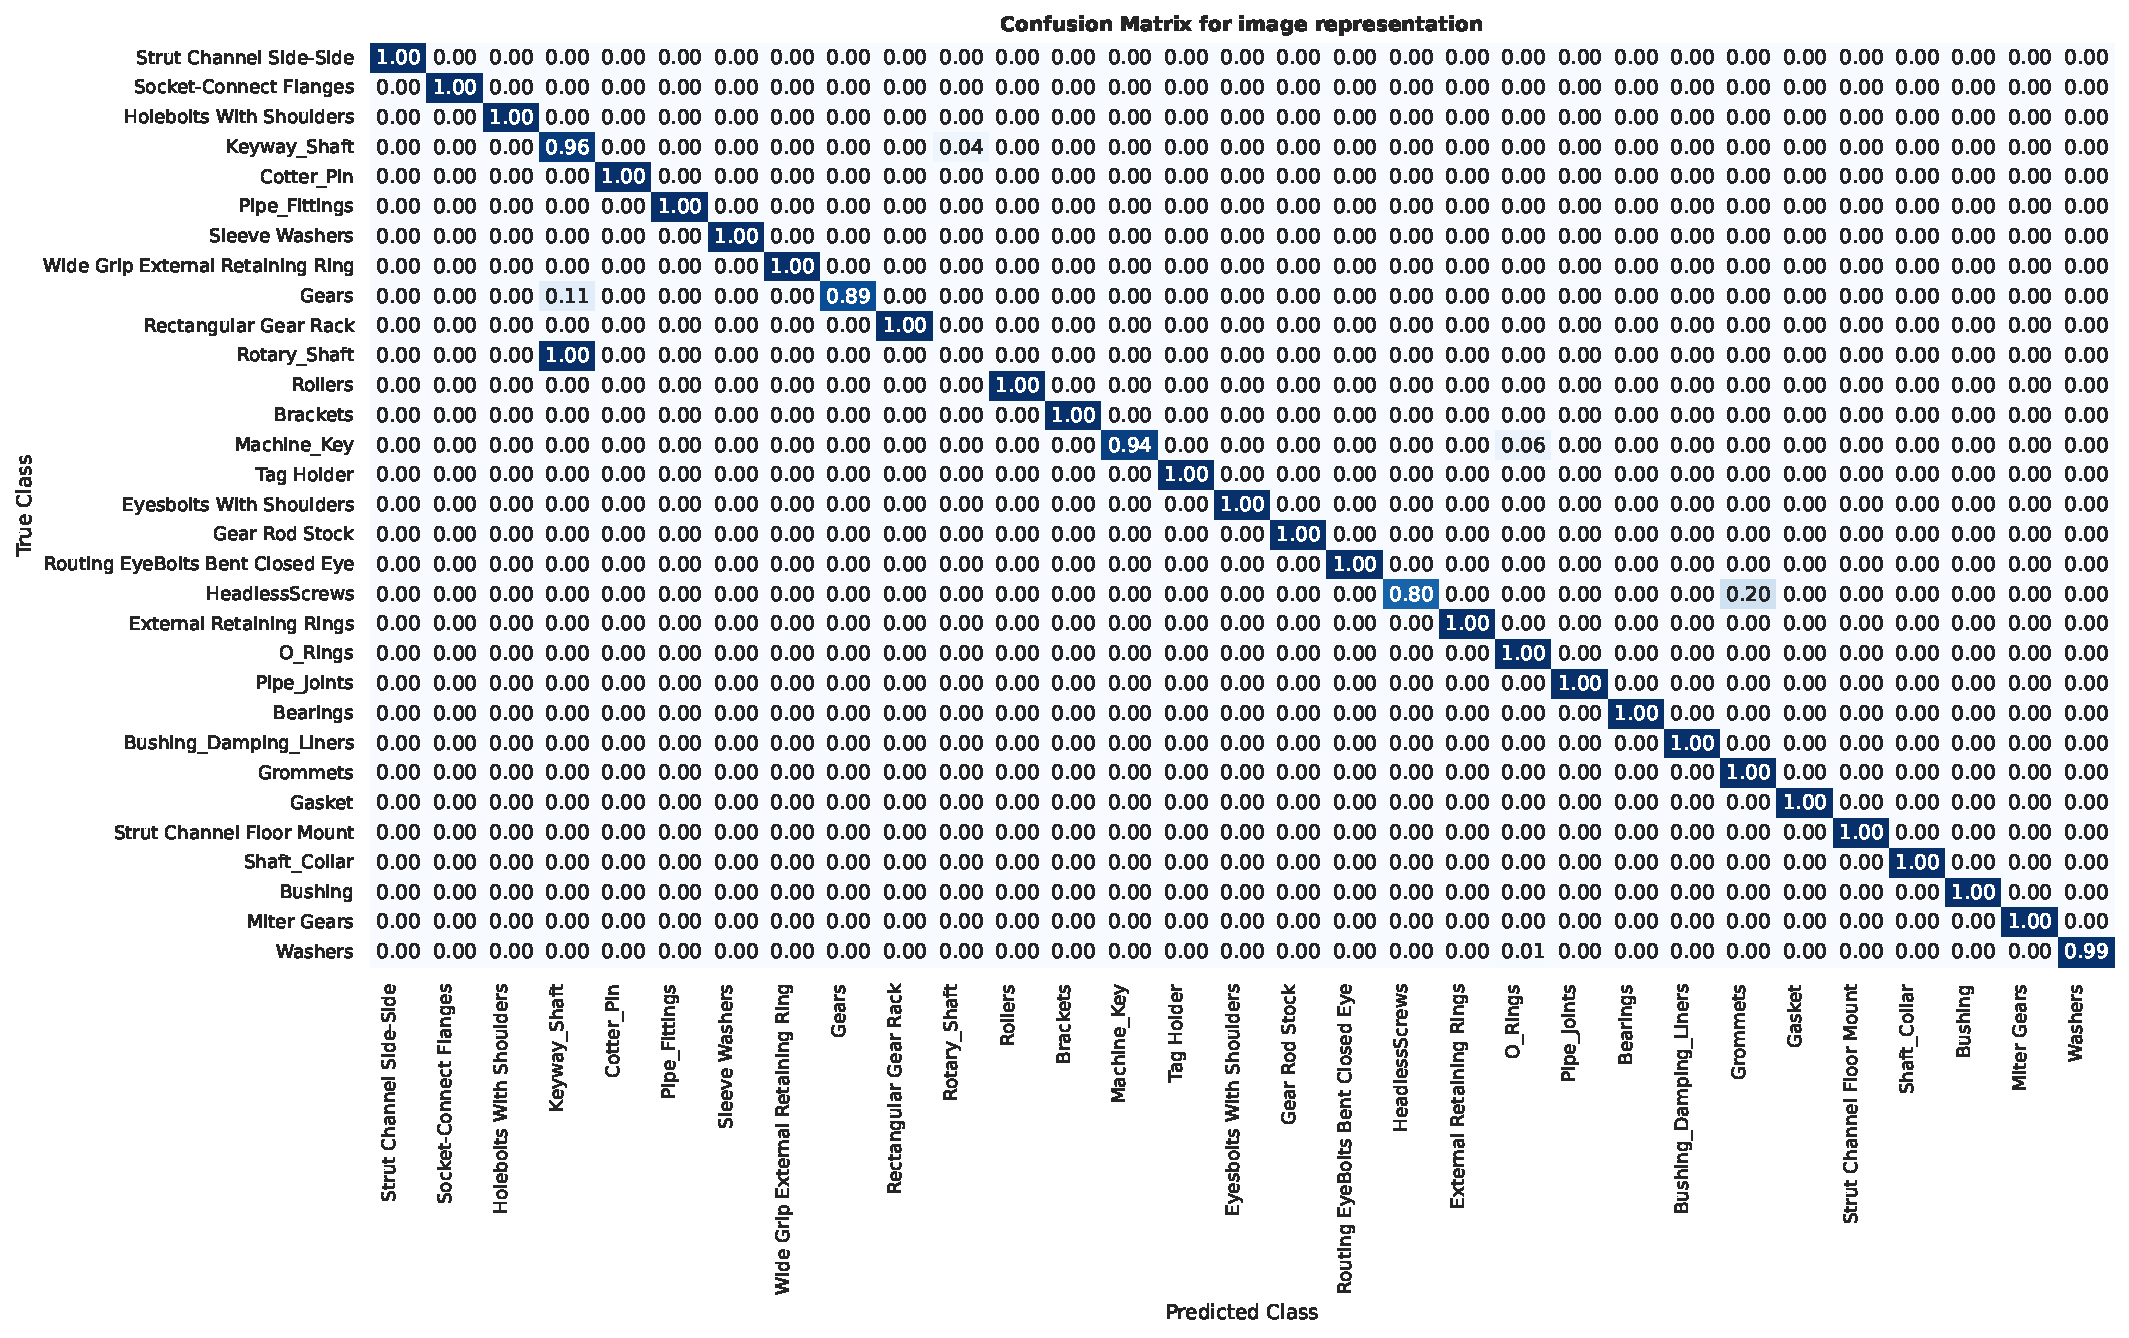
\includegraphics[width=0.9\textwidth]{confusion_matrix_images.pdf}}
\caption{\textbf{Confusion Matrix for the image-based Approach}\\For each part class, the confusion matrix shows the distribution of predicted classes. The image-based approach performs reasonably well, but it fails to recognize rotary shafts entirely}
\label{fig:confusion-matrix-images}
\end{figure*}

\begin{figure*}[h]
\centerline{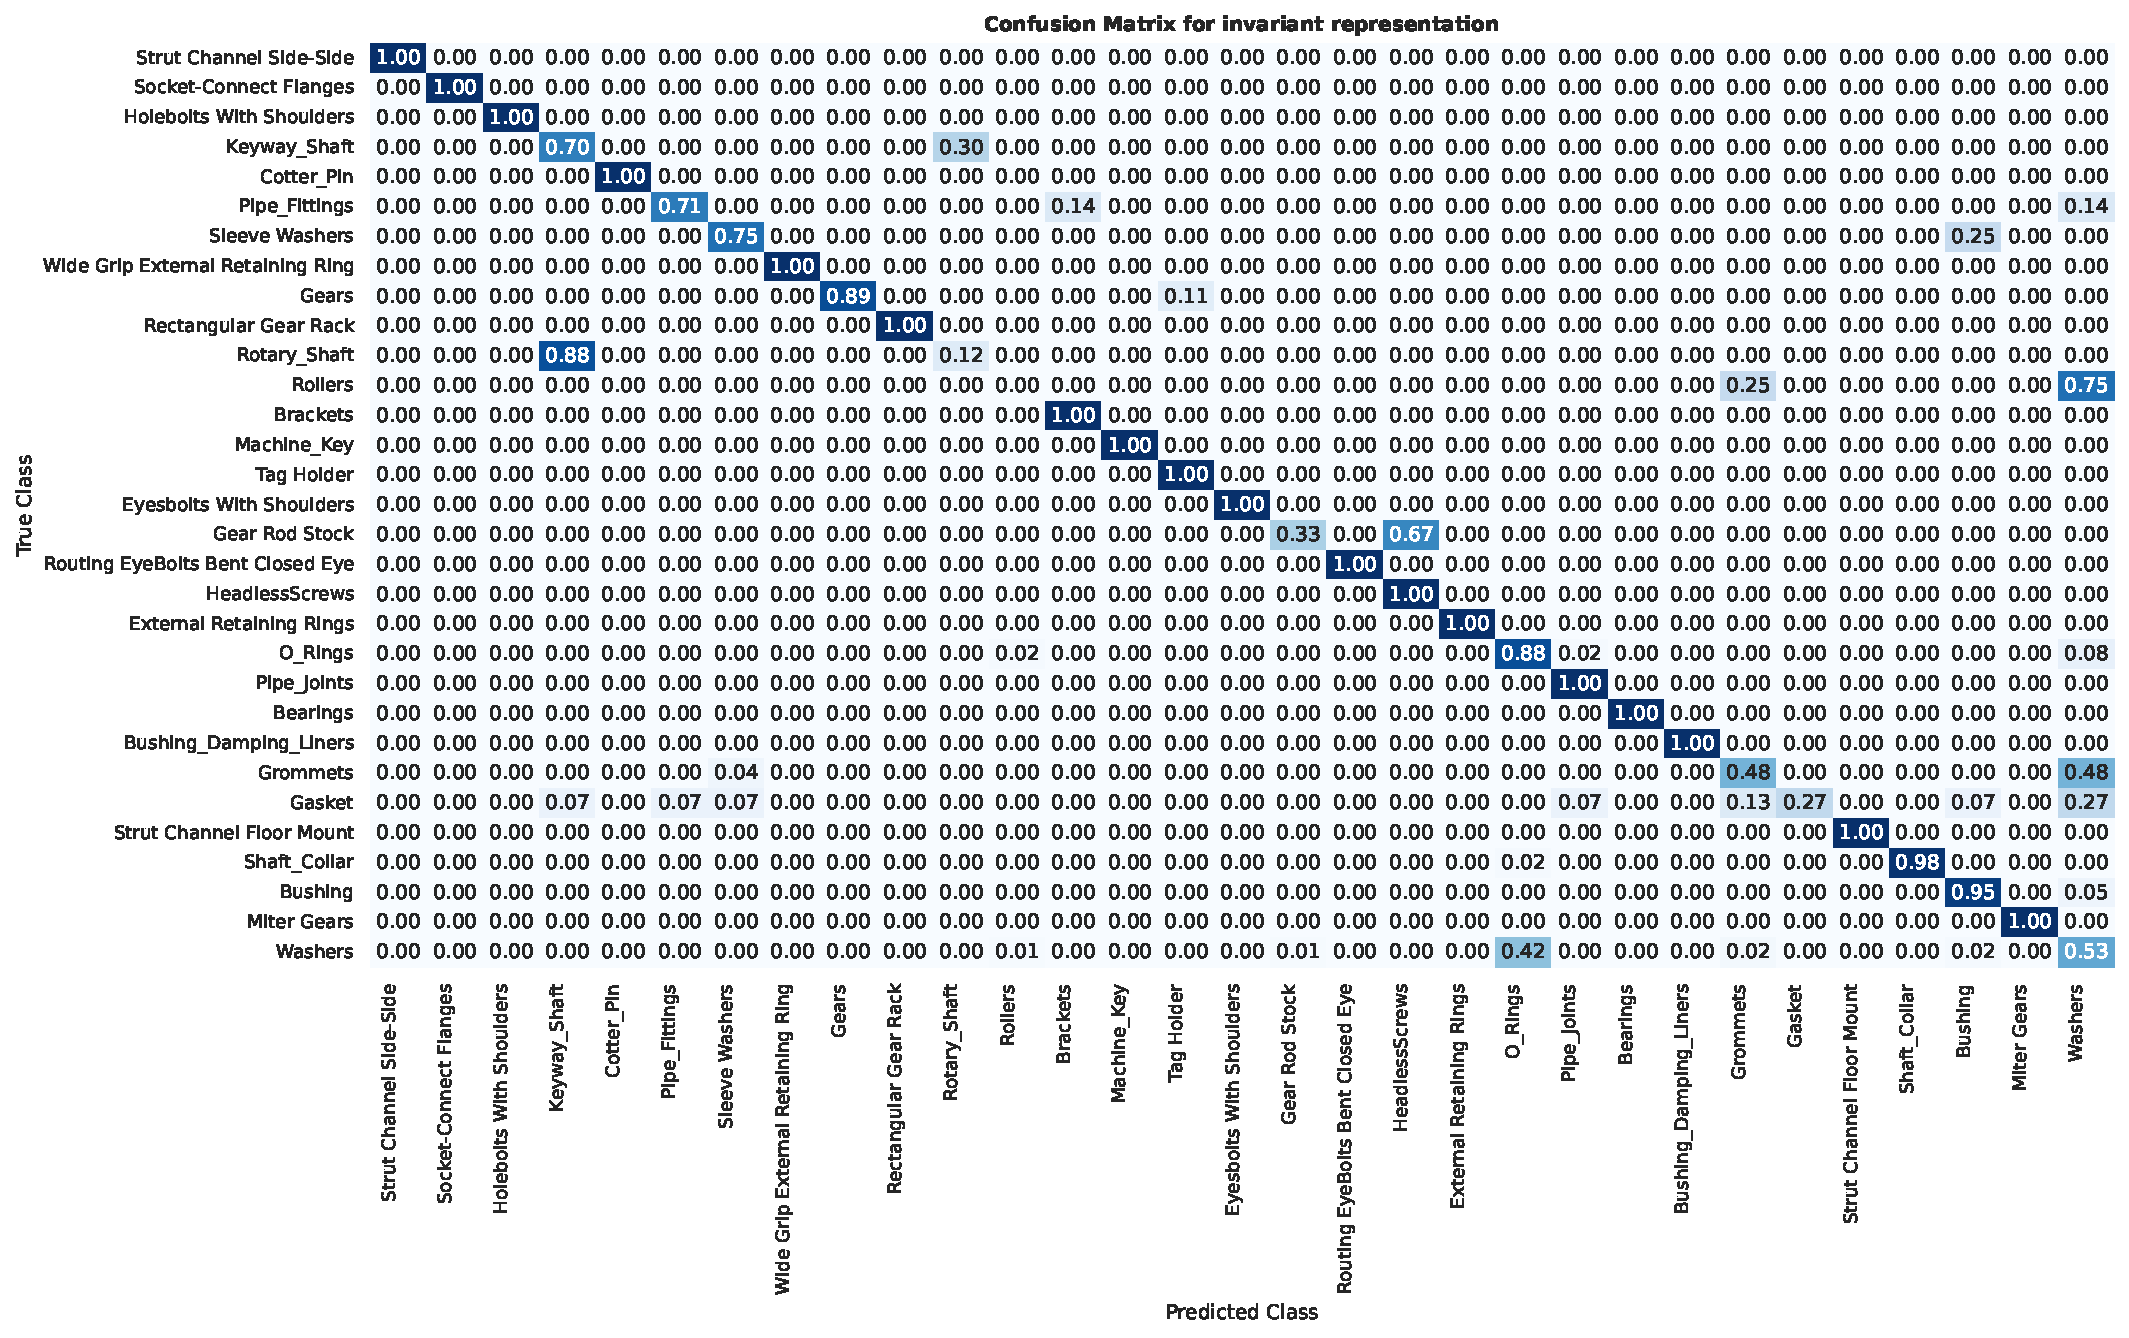
\includegraphics[width=0.9\textwidth]{confusion_matrix_invariants.pdf}}
\caption{\textbf{Confusion Matrix for the invariant-based Approach}\\For each part class, the confusion matrix shows the distribution of predicted classes. Compared to the other approaches, the invariant-based approach performs worse overall, with a significant number of misclassifications across many classes.}
\label{fig:confusion-matrix-invariants}
\end{figure*}

\begin{figure*}[h]
\centerline{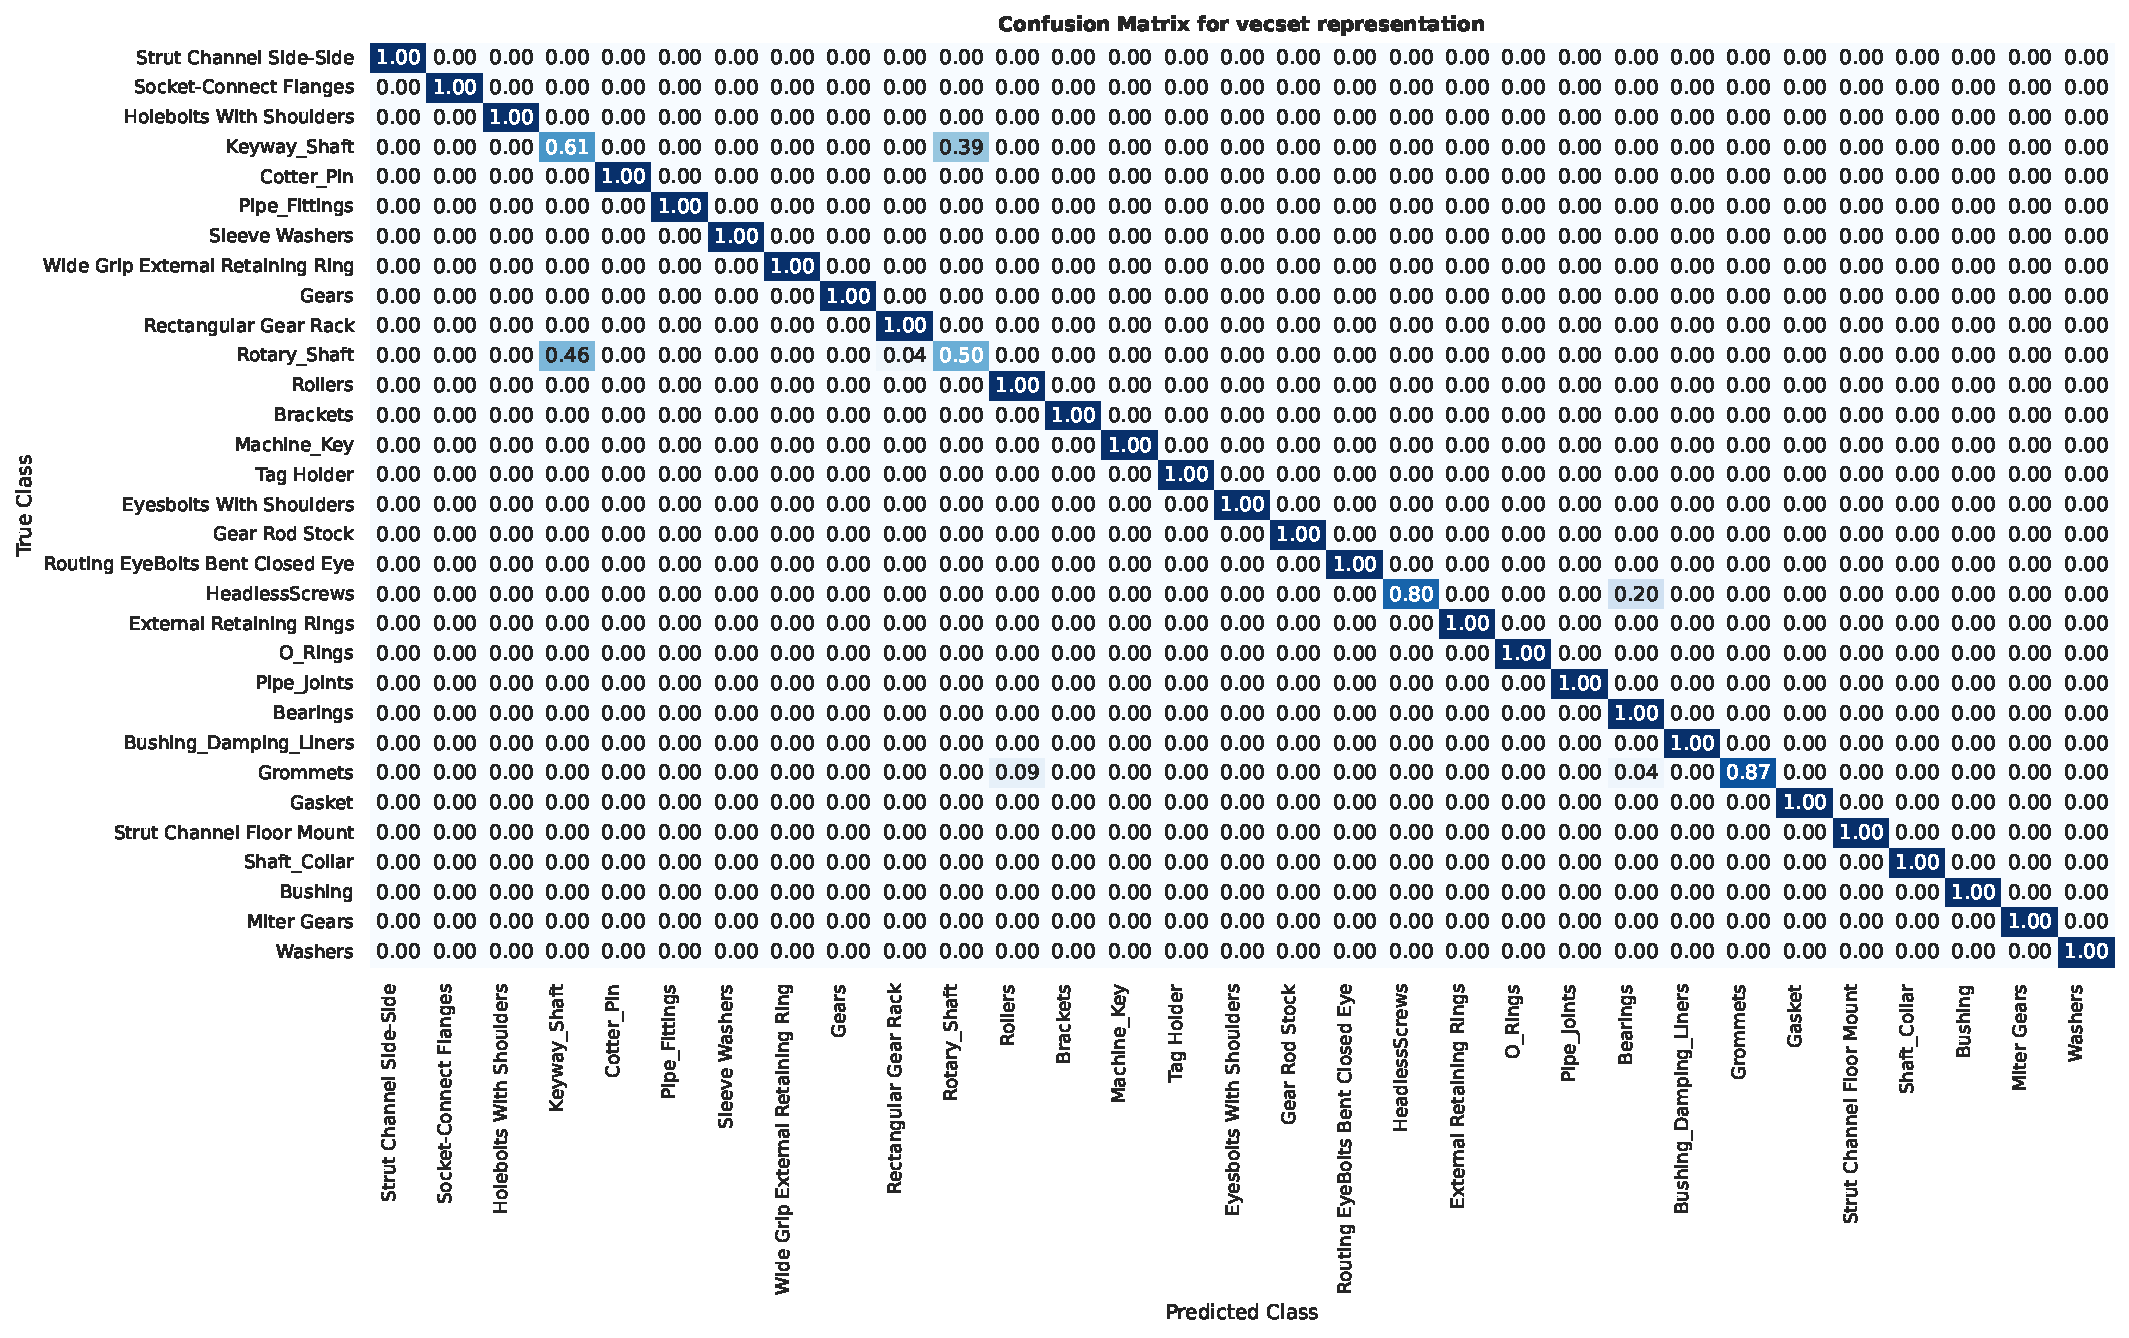
\includegraphics[width=0.9\textwidth]{confusion_matrix_vecsets.pdf}}
\caption{\textbf{Confusion Matrix for the vector-based Approach}\\For each part class, the confusion matrix shows the distribution of predicted classes. The vector-based approach performs reasonably well for most classes.}
\label{fig:confusion-matrix-vecset}
\end{figure*}

\begin{figure*}[t]
\centerline{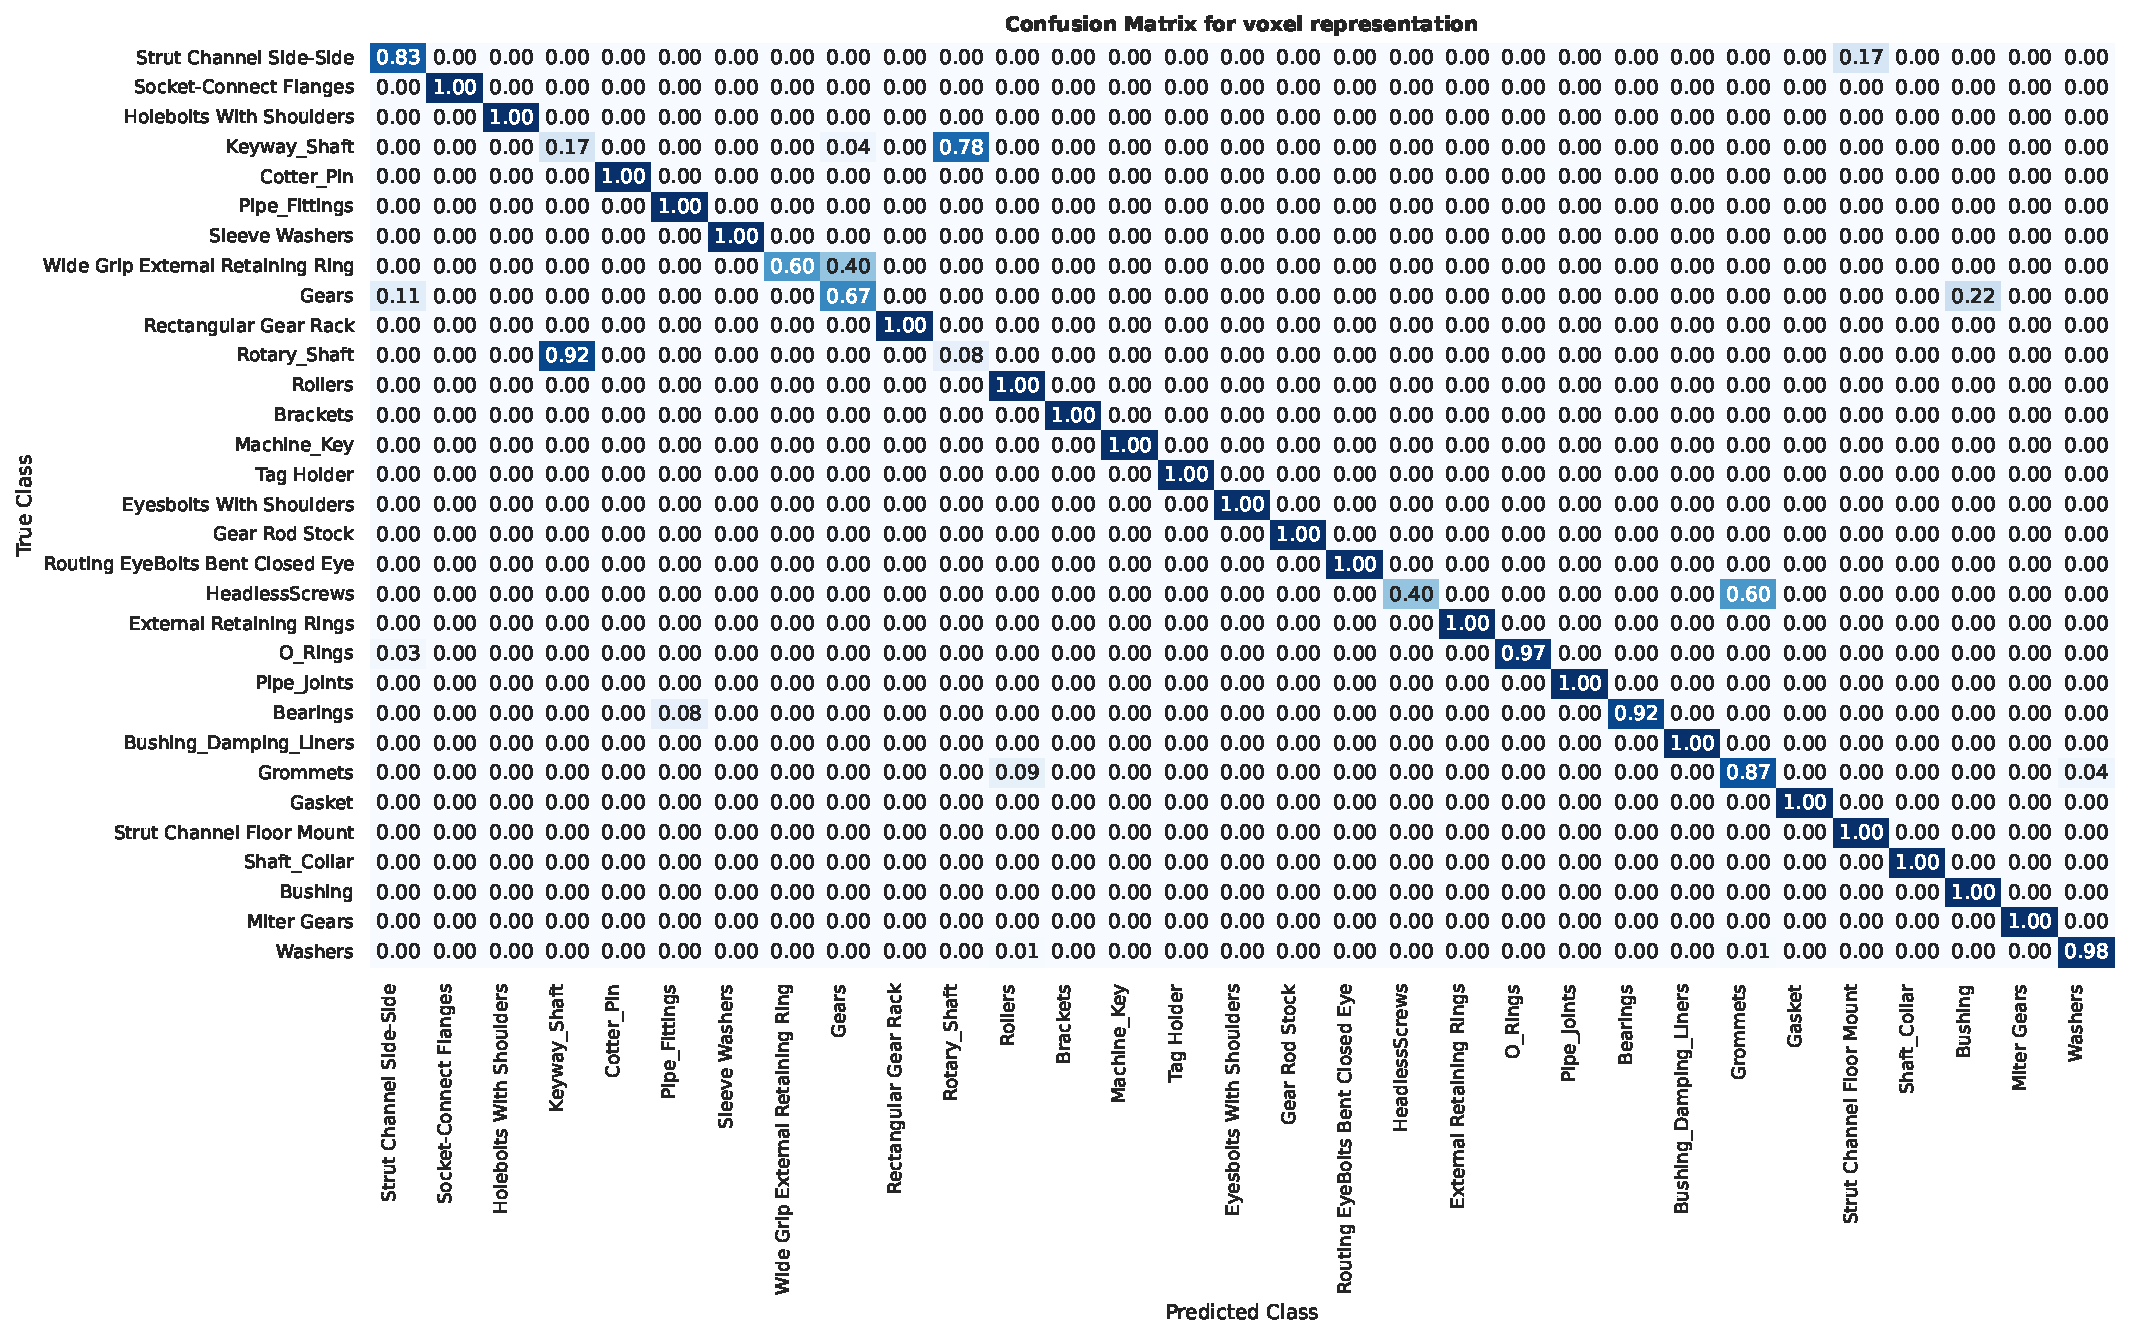
\includegraphics[width=0.9\textwidth]{confusion_matrix_voxels.pdf}}
\caption{\textbf{Confusion Matrix for the voxel-based Approach}\\For each part class, the confusion matrix shows the distribution of predicted classes. The voxel-based approach shows reasonable performance across most classes, but yields a significant number of misclassifications for some classes, especially for keyway shafts, rotary shafts and headless screws.}
\label{fig:confusion-matrix-voxels}
\end{figure*}

% Error distributions plots
\begin{figure*}[t]\vspace*{4pt}
\centerline{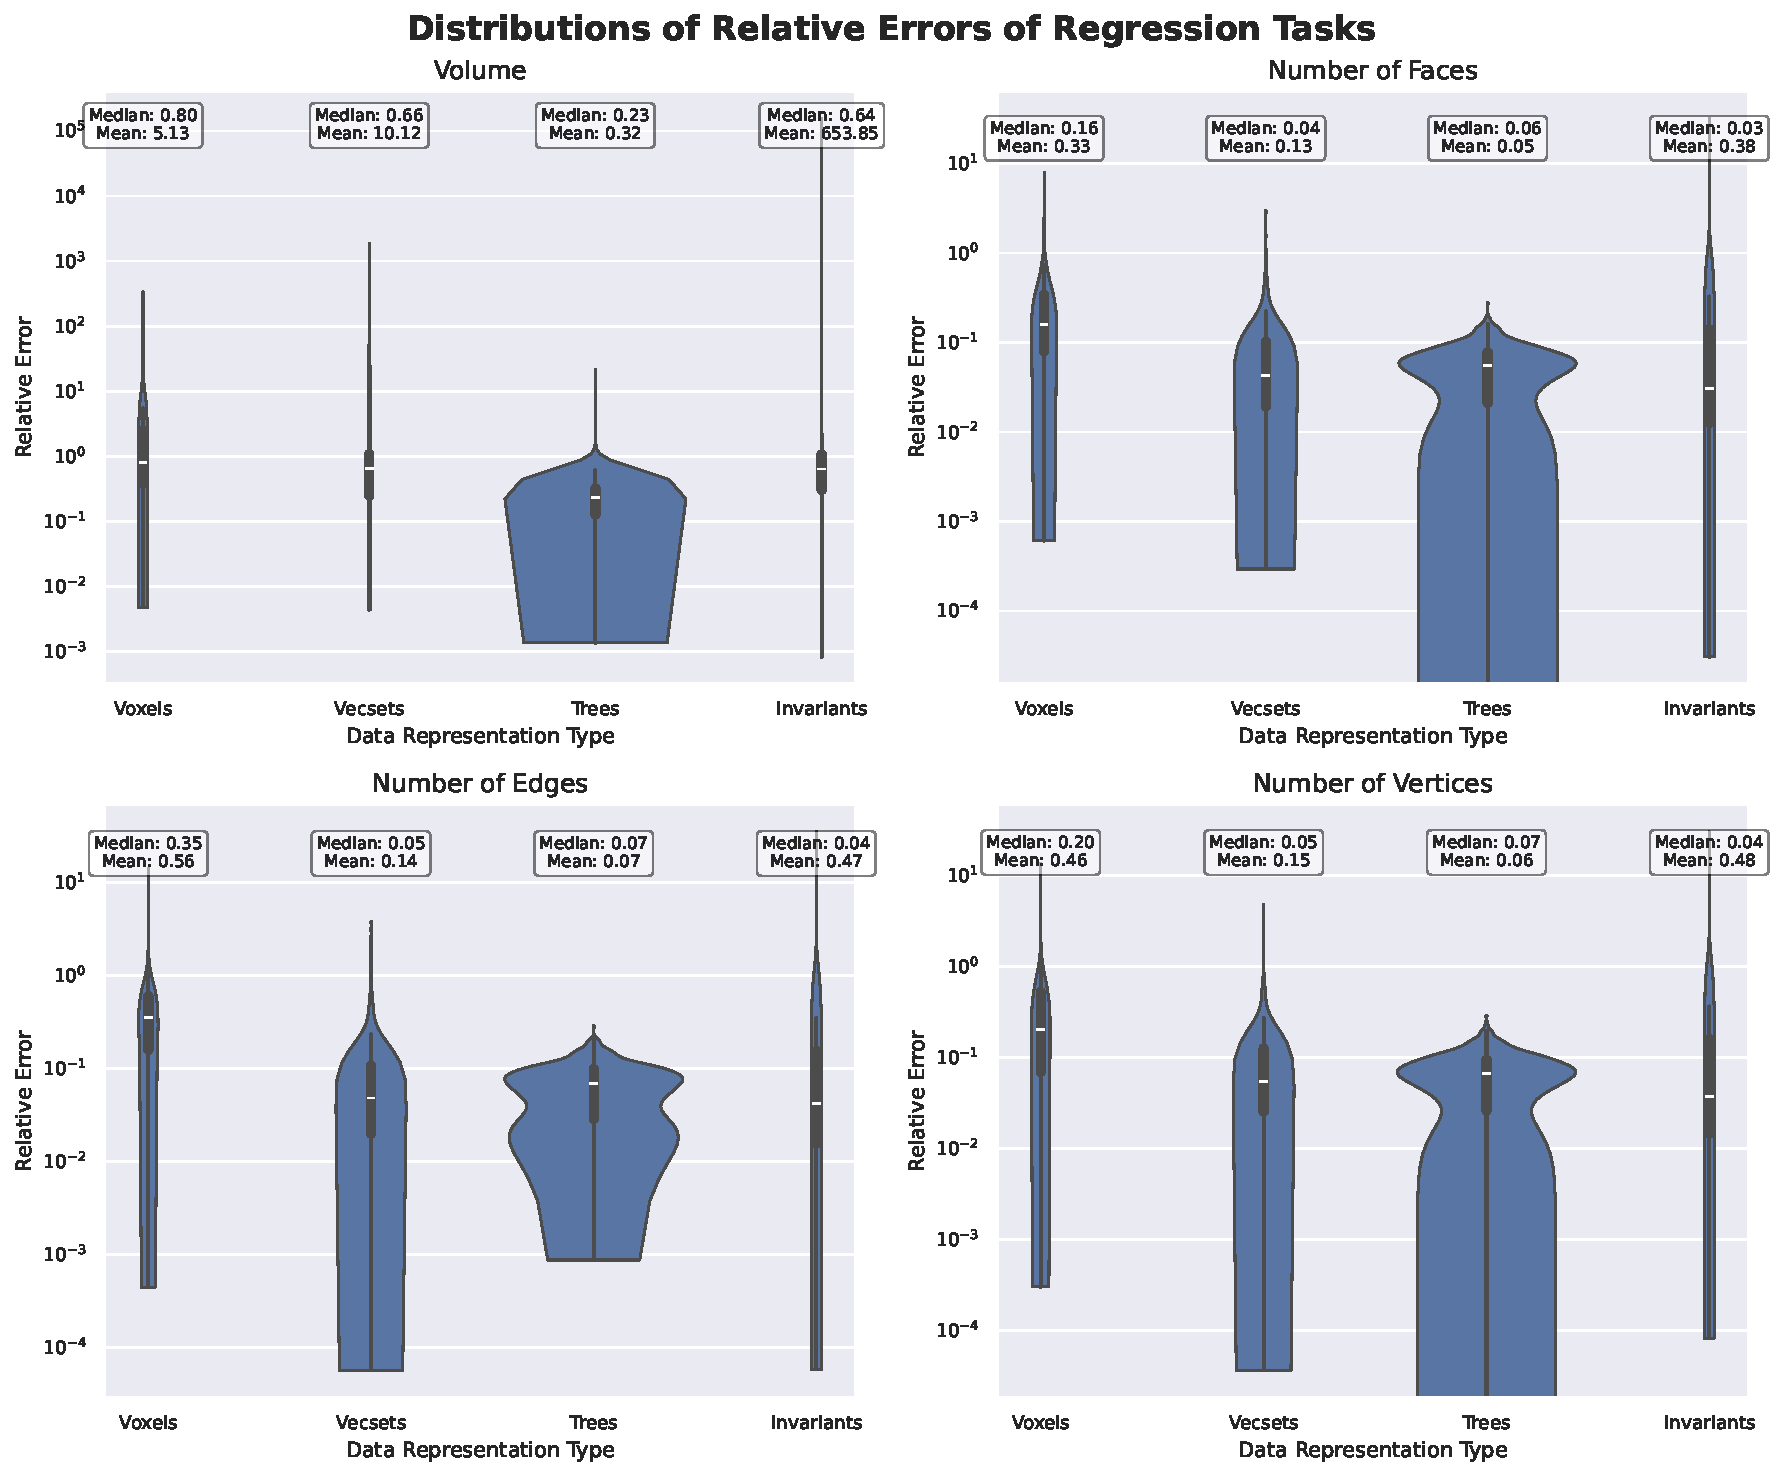
\includegraphics[width=0.9\textwidth]{error_distributions.pdf}}
\caption{\textbf{Violinplot of Error Distributions}\\Each subplot shows the distributions of the relative absolute errors for one of the regressions features and for each approach considered.
Median and mean values are provided for each distribution.
For each violinplot, the corresponding boxplot is shown as well. The whiskers of the boxplot extend to 1.5 times the interquartile range. The tree-based approach achieves the lowest mean relative error on all targets.}
\label{fig:error-distributions}
\end{figure*}

\clearpage

%  Tabelle zu Abschnitt 4.2 
\begin{table*}[t]
\centering
\caption{Regression results and reference baselines. For each target the table
reports the mean absolute error (MAE), the mean squared error (MSE), the
coefficient of determination ($R^2$) besides the median and mean of the absolute
relative error ($e_{\mathrm{rel}}$). All baselines are fitted on the oversampled
training split.}
\label{tab:regression}
\begin{tabular}{llrrrrr}
\toprule
Target & Approach & MAE & MSE & $R^2$ & med.\ $e_{\mathrm{rel}}$ & mean $e_{\mathrm{rel}}$ \\
\midrule
\multirow{7}{*}{Volume}
 & Voxels                & $4.02\cdot10^{5}$          & $1.17\cdot10^{13}$          & 0.015            & 0.81            & 5.38 \\
 & Vecsets               & $3.36\cdot10^{5}$          & $9.84\cdot10^{12}$          & 0.173            & 0.68            & 10.67 \\
 & Trees                 & $2.06\cdot10^{5}$          & $3.32\cdot10^{12}$          & 0.721            & $\mathbf{0.23}$ & $\mathbf{0.32}$ \\
 & Invariants            & $\mathbf{1.43\cdot10^{5}}$ & $\mathbf{7.47\cdot10^{11}}$ & $\mathbf{0.937}$ & 0.66            & 611.00 \\
\cmidrule(l){2-7}
 & Global mean           & $7.48\cdot10^{5}$ & $1.18\cdot10^{13}$ & $-0.000$ & 66.76 & $5.08\cdot10^{3}$ \\
 & Global median         & $4.22\cdot10^{5}$ & $1.20\cdot10^{13}$ & $-0.015$ & 0.98  & 85.00 \\
 & Class-conditional median & $2.63\cdot10^{5}$ & $3.08\cdot10^{12}$ & 0.739 & 0.82 & 30.33 \\
\midrule
\multirow{7}{*}{Faces}
 & Voxels                & 6.45            & 316.2            & 0.462            & 0.16            & 0.33 \\
 & Vecsets               & 2.84            & 128.3            & 0.782            & 0.04            & 0.12 \\
 & Trees                 & $\mathbf{1.45}$ & $\mathbf{15.3}$  & $\mathbf{0.974}$ & 0.05            & $\mathbf{0.05}$ \\
 & Invariants            & 3.31            & 166.2            & 0.717            & $\mathbf{0.03}$ & 0.32 \\
\cmidrule(l){2-7}
 & Global mean           & 16.80 & 612.0 & $-0.050$ & 1.51 & 5.38 \\
 & Global median         & 11.37 & 615.7 & $-0.056$ & 0.50 & 2.17 \\
 & Class-conditional median & 3.43 & 234.6 & 0.598 & 0.00 & 0.41 \\
\midrule
\multirow{7}{*}{Edges}
 & Voxels                & 22.13           & $3.37\cdot10^{3}$ & 0.339            & 0.37            & 0.57 \\
 & Vecsets               & 8.20            & $1.11\cdot10^{3}$ & 0.782            & 0.05            & 0.14 \\
 & Trees                 & $\mathbf{4.70}$ & $\mathbf{162.8}$  & $\mathbf{0.968}$ & 0.07            & $\mathbf{0.07}$ \\
 & Invariants            & 9.52            & $1.26\cdot10^{3}$ & 0.753            & $\mathbf{0.04}$ & 0.40 \\
\cmidrule(l){2-7}
 & Global mean           & 50.01 & 5330 & $-0.053$ & 2.04 & 7.73 \\
 & Global median         & 32.17 & 5364 & $-0.059$ & 0.75 & 2.71 \\
 & Class-conditional median & 9.41 & 2076 & 0.590 & 0.00 & 0.31 \\
\midrule
\multirow{7}{*}{Vertices}
 & Voxels                & 14.60           & $1.54\cdot10^{3}$ & 0.318            & 0.22            & 0.47 \\
 & Vecsets               & 5.50            & 507.1             & 0.776            & 0.06            & 0.15 \\
 & Trees                 & $\mathbf{3.09}$ & $\mathbf{71.6}$   & $\mathbf{0.968}$ & 0.06            & $\mathbf{0.06}$ \\
 & Invariants            & 6.33            & 552.4             & 0.756            & $\mathbf{0.04}$ & 0.42 \\
\cmidrule(l){2-7}
 & Global mean           & 33.40 & 2365  & $-0.053$ & 2.06 & 9.78 \\
 & Global median         & 21.74 & 2385  & $-0.062$ & 0.75 & 3.48 \\
 & Class-conditional median & 6.35 & 923.6 & 0.589 & 0.00 & 0.42 \\
\bottomrule
\end{tabular}
\end{table*}

 

% Plots for regression metrics: MAE, MSE and R2
\begin{figure*}[t]\vspace*{4pt}
\centerline{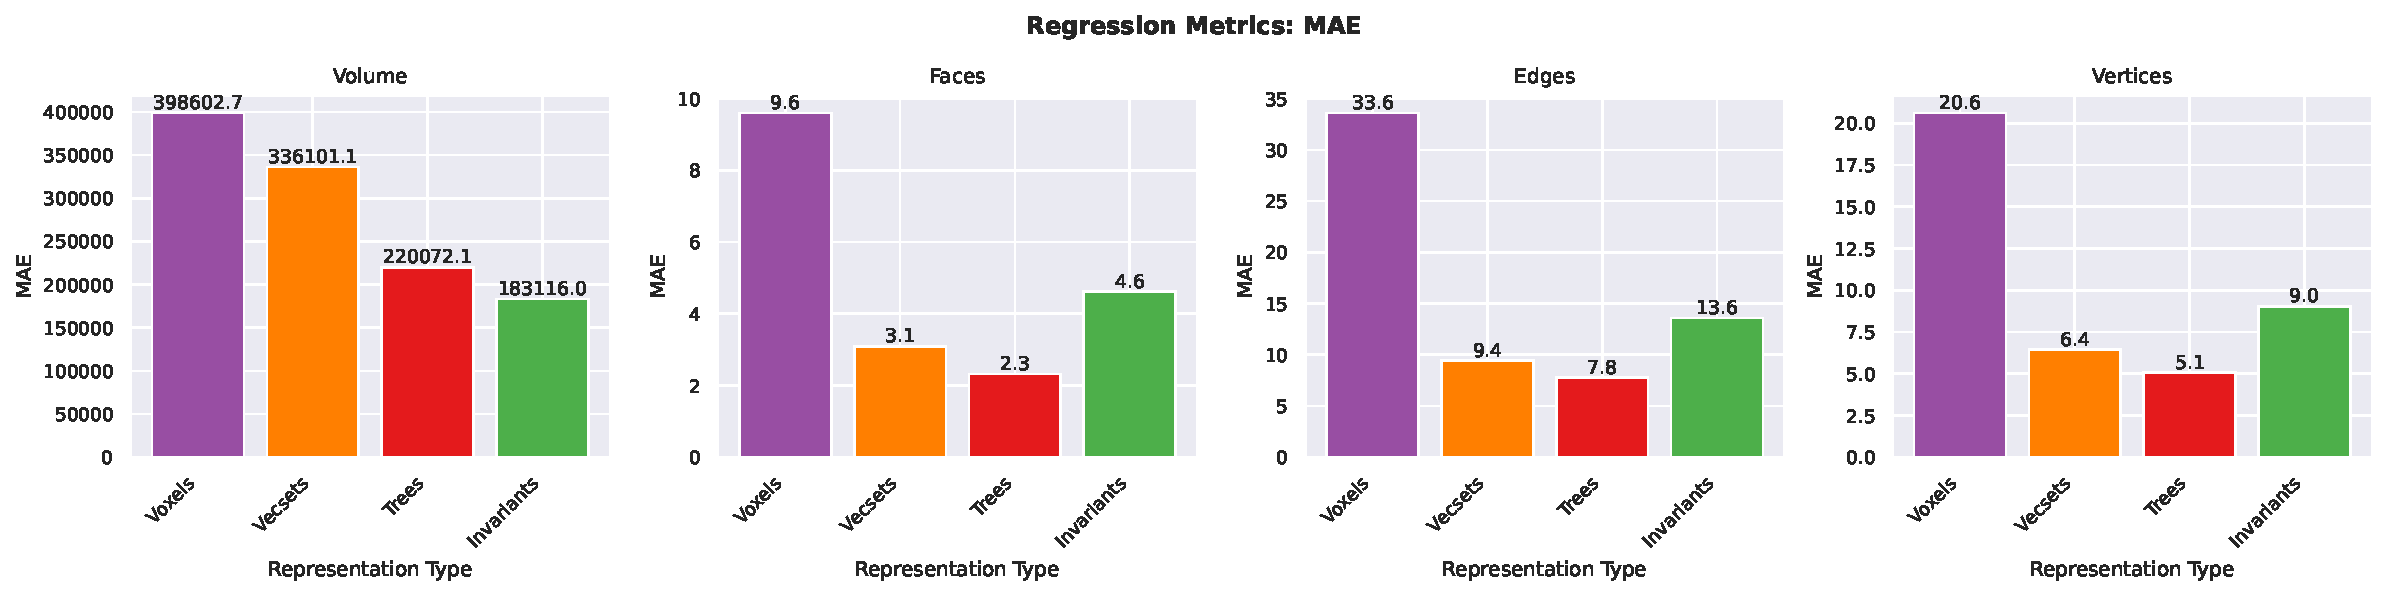
\includegraphics[width=0.9\textwidth]{regression_metrics_mae_plot.pdf}}
\caption{\textbf{Mean Absolute Errors}\\The plots show the mean absolute errors for each regression target and approach. Except for the volume target, the tree-based approach achieves the best performance across all targets.} 
\label{fig:mean-absolute-errors}
\end{figure*}

\begin{figure*}[t]\vspace*{4pt}
\centerline{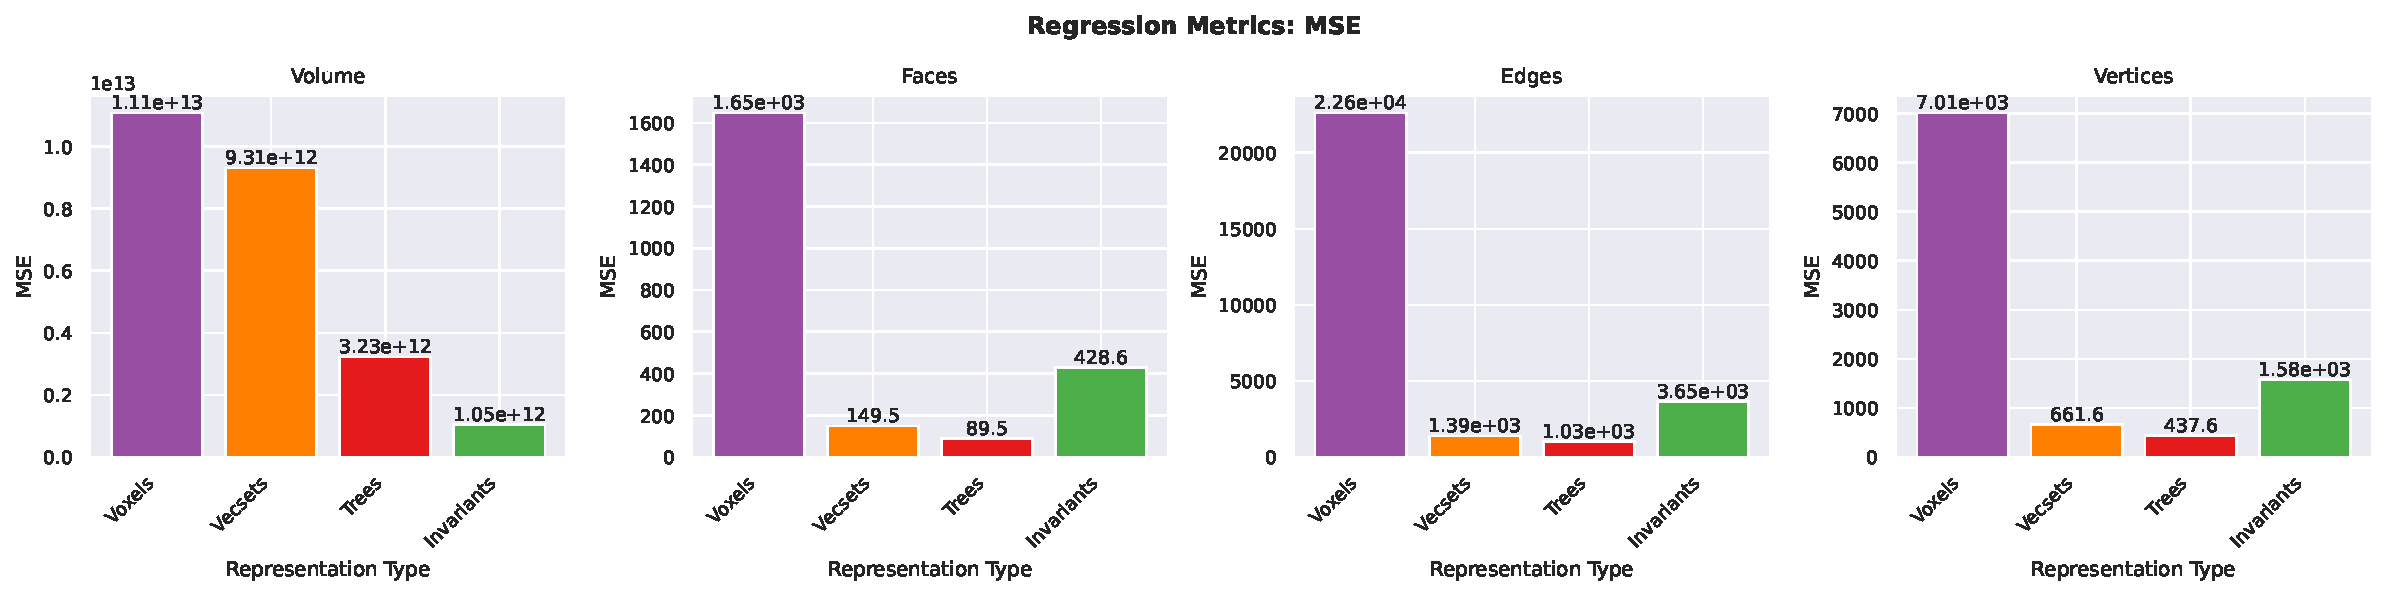
\includegraphics[width=0.9\textwidth]{regression_metrics_mse_plot.pdf}}
\caption{\textbf{Mean Squared Errors}\\The plots show the mean squared errors for each regression target and approach. Except for the volume target, the tree-based approach achieves the best performance across all targets.}
\label{fig:mean-squared-errors}
\end{figure*}

\begin{figure*}[t]\vspace*{4pt}
\centerline{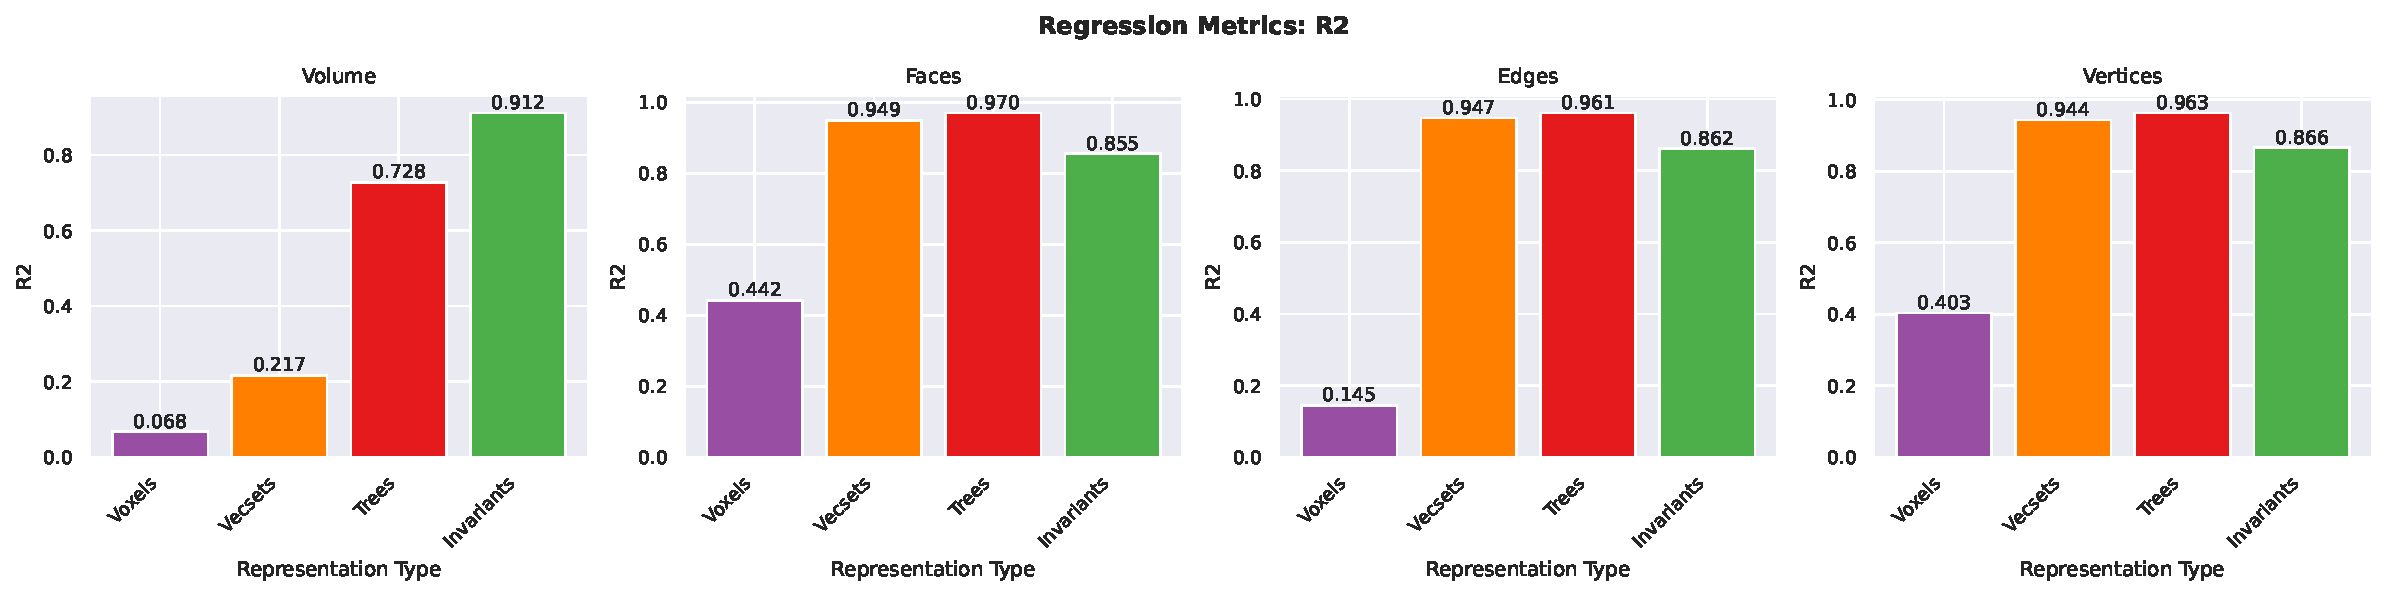
\includegraphics[width=0.9\textwidth]{regression_metrics_r2_plot.pdf}}
\caption{$\mathbf{R^2}$ \textbf{Scores}\\The plots show the $R^2$ scores for each regression target and approach. Except for the volume target, the tree-based approach achieves the best performance across all targets. On the topological targets, the voxel-based approach stays below the class-conditional median baseline of \cref{tab:regression}, whereas all other approaches exceed it.}
\label{fig:r2-scores}
\end{figure*}

\clearpage

%% References
%%
%% Following citation commands can be used in the body text:
%% Usage of \cite is as follows:
%%   \cite{key}         ==>>  [#]
%%   \cite[chap. 2]{key} ==>> [#, chap. 2]
%%

%The citation must be used in following style: \cite{article-minimal} \cite{article-full} \cite{article-crossref} \cite{whole-journal}.
%% References with BibTeX database:

%\bibliography{xampl}
%\bibliographystyle{elsarticle-harv}


%% Authors are advised to use a BibTeX database file for their reference list.
%% The provided style file elsarticle-num.bst formats references in the required Procedia style

%% For references without a BibTeX database:
\bibliographystyle{plain}
\bibliography{references}
%  \begin{thebibliography}{00}

% %% \bibitem must have the following form:
% %%   \bibitem{key}...
% %%

% \bibitem[Clark et al.(1962)]{clark}Clark, T., Woodley, R., De Halas, D., 1962. Gas-Graphite Systems, in ``{\it Nuclear Graphite}''. 
% In: Nightingale, R. (Ed.). Academic Press, New York, pp. 387.

% \bibitem[Deal and Grove(2009) ]{Deal}Deal, B., Grove, A., 1965. General Relationship for the Thermal Oxidation of Silicon. Journal of Applied Physics 36.2, 37--70.

% \bibitem[Deep(2009)]{Deep}Deep-Burn Project: Annual Report for 2009, Idaho National Laboratory, Sept. 2009.

% \bibitem[Fachinger(2004)]{Fachinger2004}Fachinger, J., den Exter, M., Grambow, B., Holgerson, S., Landesmann, C., Titov, M., Podruhzina, T., 2004. ``Behavior of spent HTR fuel elements in aquatic phases of repository host rock formations,'' 2nd International Topical Meeting on High Temperature Reactor Technology. Beijing, China, paper \#B08. 

% \bibitem[Fachinger(2006)]{Fachinger2006}Fachinger, J., 2006. Behavior
% of HTR Fuel Elements in Aquatic Phases of Repository Host Rock Formations. Nuclear Engineering \& Design 236.3,      54.

%  \end{thebibliography}

\clearpage\onecolumn
\end{document}

%%
%% End of file.
